% !TEX program = lualatex
% =====================================================================
%  WERSJA „PREZENTACJA” (kris, 22.11.2026) — jak main-promotor.tex
%  (bez \TODO, druk jednostronny), ale rozdz. 5 zawiera same wyniki
%  z parametrami pomiarów, bez interpretacji, z pustym p. „Wnioski”
%  (rozdzialy/05_badania_prezentacja.tex).
%  Kompilacja: latexmk main-prezentacja.tex
% =====================================================================
\newcommand{\wersjaPromotor}{}
\newcommand{\wersjaPrezentacja}{}
\newcommand{\interlinia}{1.25}
\documentclass[12pt, a4paper, oneside, openany]{mwrep}
% =====================================================================
%  WSPÓLNA TREŚĆ main.tex i main-roboczy.tex (wszystko po \documentclass).
%  Kolejność części i \input rozdziałów zmienia się TUTAJ.
% =====================================================================
% =====================================================================
%  WSPÓLNA PREAMBUŁA PRACY INŻYNIERSKIEJ (PWr, WEFiM)
%  Kompilacja: LuaLaTeX + biber  (latexmk -lualatex main.tex)
%  Wymogi: A4, druk dwustronny, 12 pt, Times New Roman, tekst
%  wyjustowany, rysunki/tabele/wzory numerowane w obrębie rozdziału,
%  numer strony w górnym zewnętrznym rogu.
%  Parametry do szybkiej zmiany: sekcja „USTAWIENIA” poniżej.
% =====================================================================

% ---------------------------------------------------------------------
%  USTAWIENIA
% ---------------------------------------------------------------------
% Interlinia (setspace): 1.1 w LaTeX ≈ 1,15 w Wordzie (≈ 400 słów/str.,
% zgodnie z wspolne/budzet_stron.md). 1.0 = pojedyncza, 1.25 ≈ 1,5 w Wordzie.
\providecommand{\interlinia}{1.1}

% ---------------------------------------------------------------------
%  Język i czcionki
% ---------------------------------------------------------------------
\usepackage{etoolbox}
\usepackage{fontspec}
\usepackage{polyglossia}
\setdefaultlanguage{polish}
\setotherlanguage{english}

% Times New Roman (Windows/Overleaf), w przeciwnym razie metryczny klon
% TeX Gyre Termes. Matematyka: TeX Gyre Termes Math (spójna z Times).
\usepackage{amsmath,amssymb}
\usepackage{unicode-math}
\IfFontExistsTF{Times New Roman}
  {\setmainfont{Times New Roman}}
  {\setmainfont{TeX Gyre Termes}}
\setmathfont{TeX Gyre Termes Math}
\setsansfont{TeX Gyre Heros}
\setmonofont{TeX Gyre Cursor}[Scale=MatchLowercase]
\usepackage{microtype}
\usepackage{indentfirst}   % wcięcie także pierwszego akapitu (typografia polska)

% ---------------------------------------------------------------------
%  Układ strony
% ---------------------------------------------------------------------
% Marginesy wg Golden Standard: 25 mm, od strony grzbietu 30 mm.
\usepackage[a4paper, inner=30mm, outer=25mm, top=25mm, bottom=25mm,
            headheight=15pt, headsep=6mm, footskip=12mm]{geometry}
\usepackage{setspace}
\setstretch{\interlinia}
\frenchspacing
\clubpenalty=10000 \widowpenalty=10000 \displaywidowpenalty=10000

% Numer strony w górnym zewnętrznym rogu (parzyste: lewy, nieparzyste:
% prawy), bez żywej paginy i bez stopki. Tak samo na stronach
% otwierających rozdziały.
\usepackage{fancyhdr}
\fancypagestyle{praca}{%
  \fancyhf{}%
  \fancyhead[LE,RO]{\thepage}%
  \renewcommand{\headrulewidth}{0pt}%
  \renewcommand{\footrulewidth}{0pt}}
\fancypagestyle{plain}{%
  \fancyhf{}%
  \fancyhead[LE,RO]{\thepage}%
  \renewcommand{\headrulewidth}{0pt}}
\pagestyle{praca}
% mwrep używa stylów „opening”/„closing”/„blank” na początku i końcu
% rozdziału oraz na pustych stronach — wszędzie ten sam numer strony.
\makeatletter
\let\ps@opening\ps@praca
\let\ps@closing\ps@praca
\let\ps@blank\ps@praca
\makeatother

% Spis treści do poziomu podrozdziału (x.y.z)
\setcounter{tocdepth}{2}
\setcounter{secnumdepth}{3}

% ---------------------------------------------------------------------
%  Matematyka, jednostki, chemia
% ---------------------------------------------------------------------
% Numeracja wzorów (r.n) w obrębie rozdziału, po prawej
\numberwithin{equation}{chapter}

\usepackage{siunitx}
% Jedno ustawienie dla całej pracy (słownik, p. 3.4): przecinek
% dziesiętny, mnożenie „·”, zakresy z półpauzą i jednostką raz na końcu.
\sisetup{
  output-decimal-marker = {,},
  exponent-product      = \cdot,
  group-separator       = {\,},
  group-minimum-digits  = 4,
  range-phrase          = {--},
  range-units           = single,
  list-pair-separator   = {~i~},
  list-final-separator  = {~i~},
  list-separator        = {,~},
  per-mode              = symbol,
  inter-unit-product    = \ensuremath{{}\cdot{}},
  separate-uncertainty  = true,
}
% Wsteczna zgodność: istniejące rozdziały używają \SI, \SIrange, \si, \num
% (składnia siunitx v2) — działa bez zmian. Nowy tekst: \qty, \qtyrange.

\usepackage[version=4]{mhchem}    % \ce{SiO2}, \ce{Si3N4} (opcjonalnie)

% ---------------------------------------------------------------------
%  Rysunki, tabele, wykresy, schematy
% ---------------------------------------------------------------------
\usepackage{graphicx}
\usepackage{float}
\usepackage{booktabs}
\usepackage{multirow}
\usepackage{array}
\usepackage{tabularx}
\usepackage{enumitem}
\setlist{nosep, leftmargin=*, labelindent=\parindent}
\setlist[itemize]{label=\textbullet}  % kropki zamiast półpauz (prośba autora 09.11.2026)

\usepackage{xcolor}
\usepackage{tikz}
\usetikzlibrary{arrows.meta, positioning, calc, decorations.pathmorphing}
\usepackage[european, siunitx]{circuitikz}
\usepackage{pgfplots}
\pgfplotsset{compat=1.17,
  /pgf/number format/use comma,
  /pgf/number format/1000 sep={}}

% Fragmenty-rysunki zapisane jako samodzielne dokumenty (z \documentclass
% i preambułą, np. uklad-pomiarowy/uklad_pomiarowy_body.tex) wstawia się
% makrem \inputBezPreambuly{plik} z szablon/makra.tex.

% Podpisy: „Rys. 3.1.” pod rysunkiem, „Tab. 3.1.” nad tabelą
\usepackage{caption}
\usepackage{subcaption}
\captionsetup{labelsep=period, font=small, labelfont=bf, justification=centering,
              singlelinecheck=true, skip=6pt}
\captionsetup[table]{position=top}
\captionsetup[sub]{labelformat=parens, labelsep=space, labelfont=normalfont}
\gappto\captionspolish{%
  \renewcommand{\figurename}{Rys.}%
  \renewcommand{\tablename}{Tab.}%
  \renewcommand{\bibname}{Literatura}%
  \renewcommand{\appendixname}{Załącznik}}
% numeracja rysunków i tabel w obrębie rozdziału (np. Rys. 3.1)
\counterwithin{figure}{chapter}
\counterwithin{table}{chapter}

% Ścieżki szukania grafik (względem wspolne/). Rozdziały mogą dopisywać
% własne przez \graphicspath lub makro \figdir.
\graphicspath{{rysunki/}{../}}

% ---------------------------------------------------------------------
%  Bibliografia: biblatex + biber, styl IEEE (wspolne/README.md, sekcja 3)
% ---------------------------------------------------------------------
\usepackage{csquotes}
\usepackage[backend=biber, style=ieee, sorting=none, maxnames=3, minnames=1,
            doi=false, url=false, isbn=false]{biblatex}
\addbibresource{bibliografia.bib}
% bez kropek w pozycjach: brak kropki na końcu pozycji, przecinek zamiast
% kropki między blokami (np. tytuł książki, wydawca); „nr” bez kropki
% (ściągnięcie). Skróty „t.”, „s.”, „wyd.” i inicjały zostają z kropką.
\renewcommand*{\finentrypunct}{}
\renewcommand*{\newblockpunct}{\addcomma\space}
\usepackage{regexpatch}
\makeatletter
\def\pwr@bez@kropek#1{\xpatchbibdriver*{#1}
  {\setunit{\adddot\addspace}}{\setunit{\addcomma\addspace}}{}{}}
\forcsvlist{\pwr@bez@kropek}{article,book,inbook,incollection,
  inproceedings,online,patent,report,thesis,misc,manual,collection}
\makeatother
\DefineBibliographyStrings{polish}{number={nr}, issue={nr}}

% ---------------------------------------------------------------------
%  Hiperłącza (na końcu preambuły)
% ---------------------------------------------------------------------
\usepackage[hidelinks, unicode, bookmarksnumbered, pdfusetitle]{hyperref}
\usepackage{bookmark}
% tylda i twarda spacja w zakładkach PDF (tytuły z „i~”, „w~”)
\pdfstringdefDisableCommands{\def~{ }\def\nobreakspace{ }\def\TODO#1{}}

% =====================================================================
%  WSPÓLNE MAKRA PRACY
%  Oznaczenia zgodne z wspolne/slownik.md (sekcje 3.1 i 3.3).
%  Nowe makro dopisuje się tutaj, nie w pliku rozdziału.
% =====================================================================

% ---------------------------------------------------------------------
%  Znaczniki robocze
% ---------------------------------------------------------------------
% \TODO{tekst}  — czerwona wstawka w tekście + ostrzeżenie w logu
%                 („Package praca Warning: TODO: ...”).
% W wersji do oddania ustawić w main.tex \wersjaFinalnatrue:
% każdy pozostawiony \TODO zatrzyma kompilację błędem.
% Wersja dla promotora (main-promotor.tex definiuje \wersjaPromotor przed
% \documentclass): \TODO znika z PDF (tylko ostrzeżenie w logu),
% \DOSPRAWDZENIA drukuje się zwykłym kolorem, a fragmenty objęte
% \ifwersjaPromotor\else ... \fi (puste podrozdziały) są pomijane.
\newif\ifwersjaFinalna
\newif\ifwersjaPromotor
\ifdefined\wersjaPromotor \wersjaPromotortrue \fi
\makeatletter
\newcommand{\TODO}[1]{%
  \ifwersjaFinalna
    \PackageError{praca}{Pozostawiony TODO: \detokenize{#1}}{Uzupełnij lub usuń znacznik.}%
  \else
    \PackageWarning{praca}{TODO: \detokenize{#1}}%
    \ifwersjaPromotor\unskip\else\textcolor{red}{[TODO: #1]}\fi
  \fi}
% \TODOtab{tekst} — \TODO w komórce tabeli; w wersji dla promotora „--”
\newcommand{\TODOtab}[1]{\ifwersjaPromotor --\else\TODO{#1}\fi}
\makeatother
% \DOSPRAWDZENIA{tekst} — fragment do weryfikacji (pomarańczowe tło znaczeniowe)
\newcommand{\DOSPRAWDZENIA}[1]{\ifwersjaPromotor #1\else\textcolor{orange!80!black}{#1}\fi}


% ---------------------------------------------------------------------
%  Szkic z oznaczonymi zmianami (main-szkic.tex definiuje \wersjaSzkic).
%  W pozostałych wersjach: \zm i środowiska drukują tekst zwykłym kolorem,
%  a \usun, \przen, \otwarte nie drukują nic.
%   \zm{tekst}                    — nowy lub przeredagowany fragment (niebieski)
%   \begin{zmiana}...\end{zmiana} — to samo dla całych akapitów
%   \begin{przeniesione}...\end{przeniesione} — tekst przeniesiony z innego
%                                   miejsca bez zmian treści (fioletowy)
%   \usun{opis}   — w tym miejscu usunięto fragment (czerwona notka)
%   \przen{opis}  — notka o przeniesieniu (fioletowa)
%   \otwarte{opis}— sprawa do ustalenia (pomarańczowa notka)
% ---------------------------------------------------------------------
\newif\ifwersjaSzkic
\ifdefined\wersjaSzkic \wersjaSzkictrue \fi
\definecolor{kolorZmiana}{RGB}{0,70,190}
\definecolor{kolorPrzen}{RGB}{130,0,150}
\DeclareRobustCommand{\zm}[1]{\ifwersjaSzkic{\color{kolorZmiana}#1}\else#1\fi}
\newenvironment{zmiana}{\ifwersjaSzkic\color{kolorZmiana}\fi}{}
\newenvironment{przeniesione}{\ifwersjaSzkic\color{kolorPrzen}\fi}{}
\DeclareRobustCommand{\usun}[1]{\ifwersjaSzkic{\color{red!75!black}\footnotesize\sffamily[usunięto: #1]}\fi}
\DeclareRobustCommand{\przen}[1]{\ifwersjaSzkic{\color{kolorPrzen}\footnotesize\sffamily[#1]}\fi}
\DeclareRobustCommand{\otwarte}[1]{\ifwersjaSzkic{\color{orange!85!black}\footnotesize\sffamily[DO USTALENIA: #1]}\fi}

% ---------------------------------------------------------------------
%  Odwołania (słownik, p. 5.5): małą literą, z tyldą
% ---------------------------------------------------------------------
\newcommand{\rysref}[1]{rys.~\ref{#1}}
\newcommand{\tabref}[1]{tab.~\ref{#1}}
\newcommand{\wzorref}[1]{wzór~\eqref{#1}}
\newcommand{\rozdzref}[1]{rozdz.~\ref{#1}}
\newcommand{\pref}[1]{p.~\ref{#1}}
\newcommand{\zalref}[1]{zał.~\ref{#1}}

% ---------------------------------------------------------------------
%  Terminy obcojęzyczne przy pierwszym użyciu: \ang{...} jest zajęte przez
%  siunitx (kąty), dlatego \angielski.
%  „spektroskopia EDS (\angielski{Energy Dispersive X-ray Spectroscopy})”
% ---------------------------------------------------------------------
\newcommand{\angielski}[1]{ang.~\textit{#1}}

% ---------------------------------------------------------------------
%  Rysunki i podpisy
% ---------------------------------------------------------------------
% \rysunek[szerokość]{plik}{podpis}{etykieta}
%   \rysunek[0.8\linewidth]{rozdz4/stanowisko.jpg}{Stanowisko pomiarowe
%     \opracowanieWlasne}{fig:stanowisko}
\newcommand{\rysunek}[4][\linewidth]{%
  \begin{figure}[htbp]
    \centering
    \includegraphics[width=#1]{#2}
    \caption{#3}
    \label{#4}
  \end{figure}}
% Dopiski o źródle rysunku (słownik, p. 5.10)
\newcommand{\opracowanieWlasne}{(opracowanie własne)}
\newcommand{\naPodstawie}[1]{(na podstawie~\cite{#1})}
\newcommand{\zrodlo}[1]{(źródło:~\cite{#1})}

% Tabela: podpis nad tabelą (ustawione w preambule), wzór:
% \begin{table}[htbp]\centering
%   \caption{Podpis}\label{tab:xxx}
%   \begin{tabular}{@{}lr@{}}\toprule A & B\\\midrule ... \\\bottomrule\end{tabular}
% \end{table}
% Nagłówek kolumny z jednostką: „$U_\mathrm{B}$ [\si{\volt}]” albo \tabjedn
\newcommand{\tabjedn}[2]{#1~[\si{#2}]}

% \inputBezPreambuly{plik} — wstawia fragment przygotowany jako samodzielny
% dokument (\documentclass, \usepackage, \sisetup, \begin{document} są
% pomijane; brak \end{document} nie przeszkadza). Przykład:
%   \resizebox{\textwidth}{!}{\inputBezPreambuly{../uklad-pomiarowy/uklad_pomiarowy_body}}
\makeatletter
\let\praca@begin\begin
\newcommand{\inputBezPreambuly}[1]{\begingroup
  \renewcommand{\documentclass}[2][]{}%
  \renewcommand{\usepackage}[2][]{}%
  \renewcommand{\sisetup}[1]{}%
  \def\begin##1{\ifstrequal{##1}{document}{}{\praca@begin{##1}}}%
  \input{#1}\endgroup}
\makeatother

% Domyślne katalogi z rysunkami i danymi dla fragmentów, które używają
% \figdir / \datadir (np. emisja-magnes-pomiary/emisja_tresc.tex).
% Wrapper rozdziału ustawia je przez \renewcommand przed \input.
\newcommand{\figdir}{rysunki}
\newcommand{\datadir}{dane}

% ---------------------------------------------------------------------
%  Oznaczenia wielkości (słownik, p. 3.1) — można też pisać wprost
% ---------------------------------------------------------------------
\newcommand{\UB}{U_\mathrm{B}}          % napięcie ekstrakcyjne (emiter–bramka)
\newcommand{\UT}{U_\mathrm{T}}          % napięcie przyspieszające (emiter–target)
\newcommand{\Ie}{I_\mathrm{e}}          % prąd emisji
\newcommand{\IB}{I_\mathrm{B}}          % prąd bramki
\newcommand{\IT}{I_\mathrm{T}}          % prąd targetu
\newcommand{\RT}{R_\mathrm{T}}          % rezystor w obwodzie targetu
\newcommand{\RB}{R_\mathrm{B}}          % rezystor w obwodzie bramki
\newcommand{\Ezero}{E_0}                % energia elektronów wiązki
\newcommand{\Ec}{E_\mathrm{c}}          % energia krytyczna
\newcommand{\me}{m_\mathrm{e}}          % masa elektronu
\newcommand{\kB}{k_\mathrm{B}}          % stała Boltzmanna
\newcommand{\FL}{\vec F_\mathrm{L}}     % siła Lorentza
\newcommand{\RKO}{R_\mathrm{KO}}        % zasięg Kanayi–Okayamy
\newcommand{\dd}{\mathop{}\!\mathrm{d}} % różniczka: \dd x

% Linie widmowe (notacja Siegbahna): „Si~\Ka”, „Fe~\Kb”
\newcommand{\Ka}{K\ensuremath{\alpha}}
\newcommand{\Kb}{K\ensuremath{\beta}}
\newcommand{\La}{L\ensuremath{\alpha}}

% Jednostka umowna (jasność ekranu L)
\DeclareSIUnit{\ju}{j.u.}

% Plik z dodatkowymi makrami wątków (opcjonalny)
\InputIfFileExists{szablon/makra_dodatkowe.tex}{}{}

% =====================================================================
%  STRONA TYTUŁOWA I STRESZCZENIA wg wzoru WEFiM „inz_pl_w12n.docx”
%  (wefim.pwr.edu.pl → Dyplomowanie → Zasady edytowania pracy, p. C)
%  Strona 1: uczelnia, wydział, kierunek, PRACA DYPLOMOWA INŻYNIERSKA,
%            tytuł (identyczny z USOS-APD), autor, opiekun, Wrocław rok.
%  Strona 2: Streszczenie + Słowa kluczowe, Abstract + Keywords
%            (tożsame z tekstem w USOS-APD).
%  Dane wpisuje się w frontmatter/dane_pracy.tex — tu nic nie zmieniać.
% =====================================================================

\newcommand{\stronaTytulowa}{%
  \begin{titlepage}
    \thispagestyle{empty}
    \setstretch{1.0}
    \centering
    {\Large\bfseries Politechnika Wrocławska\par}
    \vspace{2mm}
    {\large Wydział Elektroniki, Fotoniki i~Mikrosystemów\par}
    \vspace{12mm}
    {\large Kierunek studiów: \pracaKierunek\par}
    \ifdefempty{\pracaSpecjalnosc}{}{%
      {\large Specjalność: \pracaSpecjalnosc\par}}
    \vfill
    {\huge\bfseries PRACA DYPLOMOWA\\[2mm] INŻYNIERSKA\par}
    \vspace{14mm}
    {\setstretch{1.15}\LARGE\bfseries \pracaTytul\par}
    \vspace{8mm}
    {\setstretch{1.15}\large\itshape \pracaTytulEN\par}
    \vfill
    \begin{flushright}
      \large
      \begin{tabular}{@{}l@{}}
        Autor:\\[1mm]
        \textbf{\pracaAutor}\\[8mm]
        Opiekun:\\[1mm]
        \textbf{\pracaOpiekun}
      \end{tabular}
    \end{flushright}
    \vfill
    {\large Wrocław \pracaRok\par}
  \end{titlepage}
  % Strona 2 (odwrocie): streszczenia
  \thispagestyle{plain}
  \noindent{\large\bfseries Streszczenie\par}
  \vspace{2mm}
  \pracaStreszczenie\par
  \vspace{3mm}
  \noindent\textbf{Słowa kluczowe:} \pracaSlowaKluczowe\par
  \vspace{10mm}
  \begin{otherlanguage}{english}
  \noindent{\large\bfseries Abstract\par}
  \vspace{2mm}
  \pracaAbstract\par
  \vspace{3mm}
  \noindent\textbf{Keywords:} \pracaKeywords\par
  \end{otherlanguage}
  \cleardoublepage
}

% =====================================================================
%  DANE PRACY — jedyne miejsce, w którym wpisuje się metadane.
%  Tytuł, streszczenie i słowa kluczowe MUSZĄ być identyczne z USOS-APD
%  (Regulamin studiów §35 ust. 5). Rok = rok złożenia pracy (APD: 18.12.2026).
% =====================================================================
\newcommand{\pracaAutor}{Krystian Przepiórka}
\newcommand{\pracaOpiekun}{dr inż. Paweł Urbański}
\newcommand{\pracaKierunek}{Inteligentna Elektronika}
\newcommand{\pracaSpecjalnosc}{}   % pusta = wiersz „Specjalność” pominięty
\newcommand{\pracaRok}{2026}
\newcommand{\pracaTytul}{Opracowanie, wykonanie oraz badania miniaturowego
  analizatora EDS w~technologii MEMS do zastosowań kosmicznych}
% Tytuł EN z repozytorium W:\VAULT\Inzynierka\latex (body.tex, \titlen)
\newcommand{\pracaTytulEN}{Development, implementation and testing of
  a~miniature MEMS-based EDS analyzer for space applications}

% Streszczenie i abstract: wersje robocze z repozytorium
% (frontmatter/streszczenie.tex, abstract_en.tex) — do uzupełnienia o wyniki
% i ujednolicenia z tekstem w USOS-APD.
\newcommand{\pracaStreszczenie}{%
  Celem pracy jest opracowanie, wykonanie oraz badania miniaturowego
  analizatora EDS (\angielski{Energy Dispersive X-ray Spectroscopy})
  w~technologii MEMS (\angielski{Micro-Electro-Mechanical Systems}),
  przeznaczonego do zastosowań kosmicznych. W~ramach pracy zaprojektowano
  źródło elektronów wykorzystujące zjawisko emisji polowej z~nanorurek
  węglowych (CNT) wraz z~elektrodą ekstrakcyjną oraz elektrodą umożliwiającą
  przyspieszanie wiązki elektronów. Przeanalizowano możliwość zastosowania
  magnetycznego układu ogniskowania wiązki elektronów w~celu poprawy
  \zm{jej skupienia, co umożliwia pomiar z~mniejszego obszaru próbki,}
  oraz zwiększenia efektywności wzbudzania
  charakterystycznego promieniowania rentgenowskiego. Wykonano prototyp
  układu, a~jego działanie zweryfikowano eksperymentalnie z~wykorzystaniem
  spektrometru rentgenowskiego. Oceniono możliwość wykorzystania technologii
  MEMS do budowy kompaktowych analizatorów materiałowych przeznaczonych do
  zastosowań kosmicznych. Emiter CNT wytwarzał wiązkę elektronów przy
  napięciu ekstrakcyjnym powyżej ok. 800~V, z~prądem do 200~µA. Magnes
  ogniskujący skupiał wiązkę w~zwartą plamkę na ekranie luminescencyjnym.
  W~widmach zarejestrowanych przy napięciu przyspieszającym w~zakresie od 4~kV do 10~kV
  zidentyfikowano linie charakterystyczne m.in. Mg, Al, Si, Cu, Pb, Au
  i~Cr.}
% Tekst streszczenia i abstractu musi być identyczny z wpisem w USOS-APD
% (200–300 słów) — przy wpisywaniu do APD skopiować stąd 1:1.
\newcommand{\pracaSlowaKluczowe}{%
  MEMS, spektroskopia EDS, emisja polowa, nanorurki węglowe,
  ogniskowanie magnetyczne, zastosowania kosmiczne}
\newcommand{\pracaAbstract}{%
  The aim of this thesis is to develop, build and test a~miniature EDS
  (Energy Dispersive X-ray Spectroscopy) analyzer manufactured in MEMS
  (Micro-Electro-Mechanical Systems) technology, intended for space
  applications. The work covers the design of an electron source based on
  cold field emission from carbon nanotubes (CNT), combined with an
  extraction electrode and an accelerating electrode. The feasibility of
  using a~magnetic electron-beam focusing system is analyzed in order to
  \zm{improve beam focusing, which enables measurements from a~smaller
  sample area,} and to increase the efficiency of characteristic
  X-ray excitation. A~working prototype is built and verified
  experimentally using an X-ray spectrometer. The feasibility of using
  MEMS technology to build compact material analyzers for space
  applications is evaluated. The CNT emitter produced an electron beam
  at extraction voltages above approx. 800~V, with currents up to
  200~µA. The focusing magnet concentrated the beam into a~compact spot
  on the luminescent screen. Characteristic lines of, among others, Mg,
  Al, Si, Cu, Pb, Au and Cr were identified in spectra recorded at
  accelerating voltages in the range of 4--10~kV.}
\newcommand{\pracaKeywords}{%
  MEMS, EDS, field emission, carbon nanotubes, magnetic focusing,
  space applications}

% Metadane PDF
\hypersetup{pdfauthor={\pracaAutor}, pdftitle={\pracaTytul},
            pdfsubject={Praca dyplomowa inżynierska, PWr WEFiM}}


% Wersja do oddania: odkomentować — każdy pozostały \TODO da błąd kompilacji.
% \wersjaFinalnatrue

\begin{document}

% ---------------- Część wstępna (kolejność wg „Zasad edytowania pracy” WEFiM)
\stronaTytulowa                      % 1. strona tytułowa, 2–3. streszczenie i abstract
% % Podziękowania (opcjonalne; budżet: z rezerwy). Włączane w main.tex.
\chapter*{Podziękowania}
\TODO{treść podziękowań lub usunąć \input w~main.tex}
  % 4. podziękowania (opcjonalne)
\ifdefined\wersjaSzkic% Strona z legendą oznaczeń — tylko w main-szkic.tex
\clearpage
\thispagestyle{empty}
{\Large\bfseries Szkic z~oznaczonymi zmianami (26.11.2026)\par}\medskip
Wersja robocza po uwagach promotora do wersji z~13.11.2026. Numery
U1--U38 odpowiadają liście w~pliku \texttt{uwagi\_promotora\_plan.md}.
\begin{itemize}
  \item {\color{kolorZmiana}Tekst niebieski} -- fragment nowy lub przeredagowany.
  \item {\color{kolorPrzen}Tekst fioletowy} -- fragment przeniesiony z~innego
        miejsca pracy bez zmiany treści; notka
        {\color{kolorPrzen}\footnotesize\sffamily[\dots]} podaje skąd.
  \item {\color{red!75!black}\footnotesize\sffamily[usunięto: \dots]} -- w~tym
        miejscu usunięto fragment.
  \item Tekst czarny -- bez zmian względem wersji z~23.11.2026.
\end{itemize}
Największa zmiana: nowy układ rozdz.~\ref{ch:podstawy} (pięć podrozdziałów
bez podpodrozdziałów, kolejność wg propozycji promotora) oraz akapity
z~tytułem zamiast podpodrozdziałów w~rozdz.~\ref{ch:badania}.
\clearpage
\fi
\tableofcontents                     % 5. spis treści
% =====================================================================
%  WYKAZ SKRÓTÓW I OZNACZEŃ — treść z wspolne/slownik.md (sekcje 2 i 3.1).
%  Słownik jest źródłem prawdy: zmiana tam → zmiana tutaj.
% =====================================================================
\chapter*{Wykaz skrótów i~oznaczeń}   % mwrep sam dodaje go do spisu treści

{\small\setstretch{1.0}
\noindent\textbf{Skróty}\par\smallskip
\noindent
\begin{tabularx}{\linewidth}{@{}l>{\raggedright\arraybackslash}X@{}}
APXS    & spektrometr rentgenowski wzbudzany cząstkami alfa (\angielski{Alpha Particle X-ray Spectrometer})\\
CNT     & nanorurki węglowe (\angielski{Carbon Nanotubes})\\
CNT-PVP & kompozyt nanorurek węglowych i~poliwinylopirolidonu\\
DRIE    & głębokie trawienie reaktywne jonowe (\angielski{Deep Reactive Ion Etching})\\
EDS     & spektroskopia rentgenowska z~dyspersją energii (\angielski{Energy Dispersive X-ray Spectroscopy})\\
F--N    & Fowler--Nordheim (równanie, wykres)\\
FWHM    & szerokość połówkowa (\angielski{Full Width at Half Maximum})\\
KOH     & wodorotlenek potasu\\
MCA     & analizator wielokanałowy (\angielski{Multichannel Analyzer})\\
MEMS    & mikrosystemy elektromechaniczne (\angielski{Micro-Electro-Mechanical Systems})\\
NdFeB   & stop neodym--żelazo--bor (magnes trwały)\\
PIXL    & przyrząd łazika Perseverance (\angielski{Planetary Instrument for X-ray Lithochemistry})\\
PVP     & poliwinylopirolidon (\angielski{Polyvinylpyrrolidone})\\
RTG     & rentgenowski (tylko w~nazwie „źródło RTG MEMS”)\\
SDD     & krzemowy detektor dryfowy (\angielski{Silicon Drift Detector})\\
SEM     & elektronowy mikroskop skaningowy (\angielski{Scanning Electron Microscope})\\
Si(Li)  & detektor krzemowy kompensowany litem\\
TMAH    & wodorotlenek tetrametyloamoniowy (\angielski{Tetramethylammonium Hydroxide})\\
UV      & nadfiolet (\angielski{Ultraviolet})\\
WDS     & spektroskopia z~dyspersją długości fali (\angielski{Wavelength Dispersive X-ray Spectroscopy})\\
XRF     & fluorescencja rentgenowska (\angielski{X-ray Fluorescence})\\
ZAF     & poprawki na liczbę atomową (Z), absorpcję (A) i~fluorescencję (F)\\
\end{tabularx}

\newpage
\noindent\textbf{Oznaczenia}\par\smallskip
\noindent
\begin{tabularx}{\linewidth}{@{}l>{\raggedright\arraybackslash}X>{\raggedright\arraybackslash}p{22mm}@{}}
E, B, T          & emiter, bramka (elektroda ekstrakcyjna), target (górna elektroda z~otworem) & --\\
$\UB$            & napięcie ekstrakcyjne (emiter--bramka) & \si{\volt}\\
$\UT$            & napięcie przyspieszające (emiter--target) & \si{\volt}, \si{\kilo\volt}\\
$\Ie$            & prąd emisji & \si{\micro\ampere}\\
$\IB$            & prąd bramki & \si{\micro\ampere}\\
$\IT$            & prąd targetu & \si{\micro\ampere}\\
$\RT$, $\RB$     & rezystory ograniczające w~obwodzie targetu i~bramki & \si{\kilo\ohm}\\
$p$              & ciśnienie & \si{\milli\bar}, \si{\pascal}\\
$L$              & jasność świecenia ekranu (analiza obrazu) & \si{\ju}\\
$\Delta$         & nadmiar składowej niebieskiej piksela & --\\
$r_\mathrm{P}$   & współczynnik korelacji Pearsona & --\\
$\varphi$        & praca wyjścia & \si{\electronvolt}\\
$F$              & natężenie pola elektrycznego na powierzchni emitera & \si{\volt\per\metre}\\
$J$              & gęstość prądu emisji & \si{\ampere\per\metre\squared}\\
$\beta$          & współczynnik wzmocnienia pola & --\\
$d$              & odległość emiter--bramka & \si{\milli\metre}\\
$\Ezero$         & energia elektronów wiązki, $\Ezero = e\UT$ & \si{\kilo\electronvolt}\\
$\Ec$            & energia krytyczna (krawędź absorpcji) & \si{\kilo\electronvolt}\\
$U_0$            & współczynnik nadnapięcia $\Ezero/\Ec$ & --\\
$\vec B$         & indukcja magnetyczna & \si{\tesla}\\
$r_\mathrm{L}$   & promień Larmora & \si{\milli\metre}\\
$f$              & ogniskowa soczewki magnetycznej & \si{\milli\metre}\\
$R$              & zasięg elektronów (wzór Kanayi--Okayamy) & \si{\micro\metre}\\
$Z$, $A$, $\rho$ & liczba atomowa, masa atomowa, gęstość & --, g/mol, g/cm$^3$\\
$\omega$         & wydajność fluorescencji & --\\
$\varepsilon$    & średnia energia wytworzenia pary elektron--dziura & \si{\electronvolt}\\
$\bar l$         & średnia droga swobodna & \si{\milli\metre}\\
$e$, $m_\mathrm{e}$, $k_\mathrm{B}$ & ładunek elementarny, masa elektronu, stała Boltzmanna & --\\
\end{tabularx}
\par}
    % 6. wykaz skrótów i oznaczeń

% ---------------- Część zasadnicza
% Rozdział 1 — Wstęp (budżet: 2,5 str.)
% Wersja dopracowana 09.11.2026 na podstawie opcji C (zatwierdzonej 08.11.2026).
% Treść jest teraz tutaj; wstep-zagajenie/wstep_opcja_C.tex nie jest już wczytywany.
% Poprzednia wersja: rozdzialy/01_wstep_backup_2026-11-09.tex.
% Zamknięte pozycje rejestru: A9 (klucze cytowań), B9/W5 (masa źródła przypisana
% źródłu), B15/W2 (brzmienie o przyrządach w misjach), B26 (cele zawężone do
% zebranych danych — do potwierdzenia przez autora).
% 09.11 wieczorem (kris): mniej cytowań (1 na tezę), U_T = 4–11 kV bez 10–18 kV.
\chapter{Wstęp}
\label{ch:wstep}

Analiza składu pierwiastkowego jest jednym z~podstawowych badań
materiałowych. W~laboratoriach wykonuje się ją najczęściej metodą
spektroskopii EDS (\angielski{Energy Dispersive X-ray Spectroscopy})
w~elektronowym mikroskopie skaningowym (SEM)~\cite{goldstein2018sem}.
Wiązka elektronów pada na~próbkę, a~zawarte w~niej pierwiastki emitują
promieniowanie X o~energiach charakterystycznych dla każdego z~nich.
Spektrometr mierzy energie fotonów, co pozwala ustalić skład próbki.

Ten sam rodzaj badań jest potrzebny w~misjach kosmicznych, w~których
określa się skład skał i~gruntu na~powierzchni Księżyca, Marsa czy
planetoid. Sprowadzanie próbek na~Ziemię jest kosztowne i~możliwe tylko
w~nielicznych misjach, dlatego analizę wykonuje się na~miejscu,
przyrządami zamontowanymi na~lądowniku lub łaziku~\cite{gellert2015apxs}.
Spektrometry APXS łazików marsjańskich wzbudzają próbkę cząstkami alfa
i~promieniowaniem X ze źródła radioizotopowego~\cite{rieder2003apxs},
a~przyrząd PIXL łazika Perseverance -- promieniowaniem z~miniaturowej
lampy rentgenowskiej~\cite{allwood2020pixl}.

Wzbudzanie próbki bezpośrednio wiązką elektronów, tak jak w~EDS, nie
zostało dotąd zastosowane w~przyrządach wykorzystanych w~misjach.
Wymaga ono działa elektronowego, które w~mikroskopie wraz z~kolumną
elektronooptyczną i~układem próżniowym ma znaczne wymiary, masę i~pobór
mocy. Projekty miniaturowych mikroskopów SEM do badań Księżyca i~Marsa
nadal opierały się na~klasycznej kolumnie elektronowej~\cite{gaskin2012mvpsem}.
Na~powierzchni ciał pozbawionych atmosfery, takich jak Księżyc czy
planetoidy, panuje natomiast naturalna próżnia, w~której wiązka
elektronów może się rozchodzić bez osobnej komory.

Zmniejszenie wymiarów źródła elektronów umożliwia technologia MEMS
(\angielski{Micro-Electro-Mechanical Systems}), w~której wytwarza się
struktury o~wymiarach od~mikrometrów do~milimetrów. Na~Politechnice
Wrocławskiej powstały w~tej technologii m.in.\ polowe źródła elektronów,
mikropompy próżniowe i~mikroskop elektronowy~\cite{krysztof2019imaging},
a~także przyrządy przeznaczone do~misji kosmicznych~\cite{dziuban2022methane}.
Opracowano tam również miniaturowe źródło promieniowania rentgenowskiego
MEMS z~zimną katodą z~nanorurek węglowych (CNT).
Zimna katoda nie wymaga elementu grzejnego, a~struktura źródła ma masę
kilku gramów~\cite{urbanski2026phd}. Źródło to zaproponowano do~budowy
kompaktowego spektrometru XRF, w~którym próbkę wzbudza promieniowanie
X~\cite{urbanski2026xrf}.

W~niniejszej pracy rozwiązanie to wykorzystano w~inny sposób. Wiązka
elektronów, ogniskowana polem magnetycznym, pada bezpośrednio na~próbkę
umieszczoną na~targecie, a~spektrometr rejestruje promieniowanie
charakterystyczne próbki. Układ taki odpowiada metodzie EDS i~stanowi
miniaturowy analizator EDS w~technologii MEMS.

Tematyka pracy wpisuje się w~dyscyplinę automatyka, elektronika,
elektrotechnika i~technologie kosmiczne, ponieważ łączy elektronikę
układów zasilania źródła elektronów i~akwizycji widm, elektrotechnikę
wysokich napięć przyspieszających i~ogniskowania wiązki oraz
projektowanie przyrządu przeznaczonego do~misji kosmicznych.

Praca jest również zgodna z~profilem kierunku Inteligentna Elektronika.
Analizator EDS można traktować jako czujnik składu pierwiastkowego.
Wielkością mierzoną jest skład chemiczny próbki, a~sygnałem wyjściowym
widmo energii fotonów promieniowania X. Podobnie jak w~innych układach
czujnikowych, można w~nim wyróżnić element wzbudzający, czyli źródło
elektronów, element przetwarzający, czyli detektor z~torem akwizycji,
oraz układ zasilania i~sterowania, który ustala warunki pracy źródła,
m.in.\ napięcie ekstrakcyjne i~przyspieszające.

W~docelowym przyrządzie kosmicznym taki czujnik pracowałby samodzielnie,
bez bieżącego udziału operatora, ze względu na~opóźnienia łączności
z~Ziemią. Wymaga to elektroniki, która steruje emisją elektronów,
kontroluje stabilność prądu wiązki, rejestruje widmo i~wstępnie je
przetwarza, np.~rozpoznając linie charakterystyczne pierwiastków przed
wysłaniem danych. Zagadnienia te łączą mikrosystemy MEMS z~układami
pomiarowymi i~przetwarzaniem sygnałów, co odpowiada zakresowi kierunku
Inteligentna Elektronika.

\section{Cel i~zakres pracy}
\label{sec:cel}

Celem pracy jest opracowanie, wykonanie oraz badania prototypu
miniaturowego analizatora EDS w~technologii MEMS, przeznaczonego
do~zastosowań kosmicznych. Zakres pracy obejmuje część inżynierską
i~badawczą.

Część inżynierska:
\begin{itemize}
  \item zaprojektowanie elementów źródła elektronów (emitera i~bramki)
    oraz masek do~procesu technologicznego,
  \item wykonanie struktur krzemowych i~szklanych, uformowanie ostrza
    z~kompozytu CNT-PVP na~emiterze i~połączenie elementów bondingiem
    anodowym,
  \item zestawienie stanowiska pomiarowego z~komorą próżniową, zasilaniem
    wysokim napięciem i~spektrometrem rentgenowskim.
\end{itemize}

Część badawcza:
\begin{itemize}
  \item pomiary emisji polowej emitera CNT, czyli zależności prądu emisji
    od~napięcia,
  \item ocena wpływu magnesu ogniskującego na~kształt wiązki obserwowanej
    na~ekranie luminescencyjnym,
  \item rejestracja widma promieniowania X wzbudzanego wiązką elektronów
    i~identyfikacja linii charakterystycznych,
  \item ocena możliwości zastosowania technologii MEMS do~miniaturyzacji
    analizatorów EDS przeznaczonych do~zastosowań kosmicznych.
\end{itemize}

% B26: z celów usunięto wpływ geometrii bramki, średnicę wiązki w µm
% i porównanie liczby fotonów z magnesem i bez, bo brak takich danych.
% Jeśli autor je dostarczy, przywrócić odpowiednie punkty.
Badania prowadzono w~komorze próżniowej przy ciśnieniu do
\SI{1e-5}{\milli\bar}. Elementy połączono
bondingiem anodowym w~atmosferze, dlatego struktura nie jest hermetyczna.
Hermetyzacja z~mikropompą, istotna w~docelowym przyrządzie, nie wchodzi
w~zakres pracy, podobnie jak konstrukcja zasilacza wysokiego napięcia
i~detektora. Widma rejestrowano przy napięciu przyspieszającym $U_\mathrm{T}$
w~zakresie \SIrange{4}{11}{\kilo\volt}.
           % 7–8. wstęp, cel pracy
% Rozdział 2 — Podstawy teoretyczne i technologiczne (budżet: 10 str.)
% Źródło: podstawy-teoretyczne/podstawy_teoretyczne.tex
% (ma własne \chapter i \label{ch:podstawy}).
% =====================================================================
%  Podstawy teoretyczne i technologiczne (przegląd spójności 17.11.2026:
%  usunięto opisy stanowiska i pomiarów przeniesione do rozdz. 4, opis
%  przyrządów misyjnych dublujący wstęp, WDS z równaniami, bezpieczeństwo)
%  Zakres: zagadnienia P1 i P2 z listy zagadnien_do_opracowania.md,
%  bez P3 i bez punktu o absorpcji promieniowania w próbce/oknie detektora.
%  Wymaga: amsmath, siunitx (output-decimal-marker={,}), xcolor
%  Bibliografia: literatura-wstep/literatura_wstep.bib
%  Można rozbić na osobne rozdziały (np. sekcja 1 = rozdział technologiczny).
% =====================================================================
\providecommand{\TODO}[1]{\textcolor{red}{[TODO: #1]}}

\chapter{Podstawy teoretyczne i~technologiczne}
\label{ch:podstawy}

W~rozdziale opisano technologię wykonania struktur źródła elektronów,
zjawiska fizyczne wykorzystywane w~analizatorze (emisję polową,
przyspieszanie i~ogniskowanie wiązki, powstawanie promieniowania X)
oraz zasady pomiaru widma metodą EDS.

% =====================================================================
\section{Technologia wykonania struktur MEMS}
\label{sec:technologia}

\subsection{Materiały i~utlenianie termiczne krzemu}

Podstawowymi materiałami struktury są krzem monokrystaliczny i~szkło
borokrzemowe. Stosuje się płytki krzemowe o~orientacji (100), ponieważ
w~procesie trawienia anizotropowego ściany wnęk i~otworów tworzą się
wtedy wzdłuż płaszczyzn (111) pod przewidywalnym kątem.
Krzem jest jednocześnie materiałem konstrukcyjnym i~przewodzącym,
dlatego wytworzone z~niego elementy mogą pełnić rolę elektrod.

Szkło borokrzemowe (np. Borofloat~33 lub Pyrex) ma współczynnik
rozszerzalności cieplnej zbliżony do krzemu (ok.
\SI{3.3e-6}{\per\kelvin} wobec ok. \SI{2.6e-6}{\per\kelvin} dla Si),
dzięki czemu połączenie krzem--szkło nie pęka po ochłodzeniu.
Zawiera ono jony sodu Na$^+$, które są niezbędne w~procesie bondingu
anodowego (p.~\ref{subsec:bonding}). Szkło służy też jako izolator
między elektrodami pracującymi przy różnych potencjałach.

Warstwę tlenku krzemu SiO$_2$ wytwarza się przez utlenianie płytki
w~piecu w~temperaturze \SIrange{900}{1200}{\celsius}, w~atmosferze
suchego tlenu lub pary wodnej (utlenianie mokre, szybsze). Wzrost
warstwy opisuje model Deala--Grove'a. Na każdy nanometr tlenku zużywa
się ok. \SI{0.44}{\nano\metre} krzemu. Warstwa SiO$_2$ pełni rolę
maski podczas trawienia oraz izolatora elektrycznego. W~roztworach KOH
lepszą maską jest azotek krzemu Si$_3$N$_4$, który praktycznie się
w~nich nie trawi.

\subsection{Fotolitografia i~trawienie krzemu}

Fotolitografia przenosi wzór z~maski na powierzchnię płytki. Proces
obejmuje:
\begin{enumerate}
  \item nałożenie warstwy fotorezystu metodą wirowania,
  \item wstępne wygrzanie w~celu odparowania rozpuszczalnika,
  \item naświetlenie promieniowaniem UV przez maskę,
  \item wywołanie, czyli rozpuszczenie naświetlonych (rezyst pozytywowy)
        albo nienaświetlonych (rezyst negatywowy) obszarów,
  \item przeniesienie wzoru do warstwy maskującej (np. wytrawienie
        odsłoniętego SiO$_2$ w~buforowanym roztworze HF),
  \item usunięcie fotorezystu.
\end{enumerate}
W~strukturach źródła fotolitografia wyznacza położenie i~wymiary wnęk
i~otworów w~elektrodach.

\label{subsec:koh}

Wodny roztwór wodorotlenku potasu (typowo \SIrange{30}{40}{\percent},
\SIrange{70}{85}{\celsius}) trawi krzem z~szybkością zależną od
orientacji krystalograficznej. Płaszczyzny (100) trawią się z~szybkością
rzędu \SI{1}{\micro\metre\per\minute}, a~płaszczyzny (111) wielokrotnie
wolniej (stosunek rzędu 100:1 i~więcej). W~efekcie w~płytce (100) powstają
wnęki o~ścianach nachylonych pod kątem \ang{54.74} do powierzchni,
ograniczone płaszczyznami (111).

Właściwość ta jest wykorzystywana do wytwarzania wnęk o~zadanej
głębokości (trawienie przerywa się po określonym czasie) oraz otworów
przechodzących przez całą płytkę~\cite{urbanski2026phd}. Samo ostrze
emitera nie jest kształtowane w~krzemie, lecz formowane z~nanorurek
węglowych (p.~\ref{subsec:cnt}).
Zamiast KOH można stosować TMAH (wodorotlenek tetrametyloamoniowy), który
nie wprowadza jonów potasu, ale trawi wolniej.

Trawienie izotropowe (np. krzemu w~mieszaninie HF/HNO$_3$/CH$_3$COOH,
szkła w~kwasie fluorowodorowym HF) przebiega jednakowo we wszystkich
kierunkach i~daje zaokrąglone kształty.
Trawienie suche, w~tym głębokie trawienie reaktywne jonowe DRIE (proces
Boscha), pozwala uzyskać pionowe ściany niezależnie od orientacji
kryształu, ale wymaga drogiej aparatury. Trawienie w~KOH jest tanie
i~wystarczające dla geometrii stosowanych w~źródle, dlatego jest
podstawową metodą kształtowania krzemu w~tej pracy.

\subsection{Formowanie emitera CNT i~bonding anodowy}
\label{subsec:cnt}

W~źródłach MEMS opracowanych na Politechnice Wrocławskiej emiter ma
postać mikroostrza z~kompozytu nanorurek węglowych
i~poliwinylopirolidonu (CNT-PVP), formowanego z~zawiesiny nanorurek
na nagrzanym podłożu~\cite{urbanski2026phd}. Polimer wiąże nanorurki
ze sobą i~z~podłożem, a~na powierzchni ostrza pozostaje wiele
wystających końców nanorurek, które działają jako punkty emisji.
Emiter musi wytrzymać temperaturę i~pole elektryczne występujące
podczas bondingu anodowego. Sposób formowania ostrza w~prototypie
opisano w~\pref{sec:nanoszenie-cnt}.

\label{subsec:bonding}

Bonding anodowy łączy krzem ze szkłem zawierającym jony alkaliczne.
Metodę opisali po raz pierwszy Wallis i~Pomerantz~\cite{wallis1969anodic}.
Płaskie i~czyste powierzchnie krzemu i~szkła dociska się do siebie,
podgrzewa do ok. \SIrange{300}{450}{\celsius} i~przykłada napięcie rzędu
setek woltów (krzem jako anoda). W~tej temperaturze jony Na$^+$ w~szkle
stają się ruchliwe i~przemieszczają się w~stronę katody. Przy granicy
z~krzemem pozostaje warstwa zubożona w~sód, z~nieskompensowanym ładunkiem
ujemnym jonów tlenu. Silne pole elektrostatyczne dociska powierzchnie
do kontaktu na poziomie atomowym i~powstają wiązania Si--O--Si. Złącze
jest wytrzymałe mechanicznie i~szczelne.

\paragraph{Bonding w~próżni (rozwiązanie docelowe).}
Aby wnętrze struktury było zamknięte w~próżni, ostatnie połączenie
wykonuje się w~komorze próżniowej, przy ciśnieniu rzędu
\SI{1e-5}{\milli\bar} lub niższym~\cite{urbanski2026phd}. Proces ten
jest trudniejszy niż bonding w~atmosferze. W~próżni nie ma przewodzenia
ciepła przez gaz, więc łączone elementy nagrzewają się słabiej niż płyta
grzejna (w~pracy~\cite{urbanski2026phd} zmierzono ok.
\SIrange{250}{300}{\celsius} przy płycie nagrzanej do
\SI{450}{\celsius}). Spada wtedy przewodność jonowa szkła i~prąd
bondingu, co prowadzi do nieszczelności. Ponadto podczas bondingu i~późniejszej pracy ze ścianek wydzielają się
gazy, dlatego w~strukturze hermetycznej potrzebny jest element
podtrzymujący próżnię, np. zintegrowana mikropompa jonowo-sorpcyjna
\cite{grzebyk2014micropump,grzebyk2017pumps}.

Prototyp opisany w~tej pracy połączono bondingiem anodowym w~atmosferze,
więc nie jest on hermetyczny (\pref{sec:bonding-montaz}). Hermetyzację
przez bonding w~próżni przewiduje się jako kolejny etap rozwoju
przyrządu.

% =====================================================================
\section{Emisja elektronów}
\label{sec:emisja}

\subsection{Mechanizmy emisji i~emitery z~nanorurek węglowych}

Elektrony przewodnictwa w~metalu lub półprzewodniku są utrzymywane
w~materiale przez barierę potencjału. Minimalną energię potrzebną do
wyprowadzenia elektronu z~poziomu Fermiego do próżni nazywa się pracą
wyjścia $\varphi$. Dla większości metali i~dla węgla wynosi ona
\SIrange{4}{5}{\electronvolt}. Elektron może opuścić materiał na trzy
sposoby:
\begin{itemize}
  \item \textbf{termoemisja} -- elektron uzyskuje energię większą od
        $\varphi$ dzięki wysokiej temperaturze. Gęstość prądu opisuje
        równanie Richardsona--Dushmana
        \begin{equation}
          J = A_\mathrm{G}\,T^2 \exp\!\left(-\frac{\varphi}{k_\mathrm{B}T}\right),
        \end{equation}
        gdzie $A_\mathrm{G}$ jest stałą materiałową (dla idealnego metalu
        \SI{1.2e6}{\ampere\per\metre\squared\per\kelvin\squared}).
        Katody termoemisyjne pracują w~temperaturze ok.
        \SI{2000}{\kelvin} lub wyższej i~pobierają znaczną moc
        grzania;
  \item \textbf{fotoemisja} -- energię dostarcza foton o~energii
        $h\nu > \varphi$;
  \item \textbf{emisja polowa} -- silne pole elektryczne zwęża barierę
        potencjału na tyle, że elektrony przechodzą przez nią na drodze
        tunelowania kwantowego, bez dostarczania ciepła.
\end{itemize}
W~zastosowaniach kosmicznych i~w~strukturach MEMS korzystna jest emisja
polowa: katoda nie wymaga grzania, pracuje w~temperaturze otoczenia,
a~prąd emisji można szybko zmieniać napięciem~\cite{parmee2015cntxray}.

Zależność gęstości prądu emisji polowej od natężenia pola $F$ na
powierzchni emitera podali Fowler i~Nordheim~\cite{fowler1928emission}.
W~uproszczonej postaci:
\begin{equation}
  J = \frac{a F^2}{\varphi}\exp\!\left(-\frac{b\,\varphi^{3/2}}{F}\right),
  \label{eq:fn}
\end{equation}
gdzie $a \approx \SI{1.54e-6}{\ampere\electronvolt\per\volt\squared}$,
$b \approx 6{,}83\cdot10^{9}\ \mathrm{eV^{-3/2}\,V\,m^{-1}}$.
Do istotnej emisji potrzebne są pola rzędu
\SIrange{1e9}{1e10}{\volt\per\metre}. Takich pól nie uzyskuje się
w~płaskim układzie elektrod przy napięciach rzędu kilowoltów, ale
powstają one lokalnie na ostrych wierzchołkach.

Wzmocnienie lokalnego pola opisuje współczynnik $\beta$:
\begin{equation}
  F = \beta\,\frac{U}{d},
\end{equation}
gdzie $U$ jest napięciem między emiterem a~elektrodą ekstrakcyjną
(bramką), a~$d$ odległością między nimi. Dla ostrza o~promieniu
wierzchołka $r$ i~wysokości $h$ współczynnik $\beta$ jest w~przybliżeniu
proporcjonalny do $h/r$. Dla nanorurek węglowych $\beta$ osiąga wartości
rzędu setek do tysięcy.

Po podstawieniu $F=\beta U/d$ do~\eqref{eq:fn} i~przemnożeniu przez
efektywną powierzchnię emisji otrzymuje się zależność prądu emisji od
napięcia. Prąd jest pomijalnie mały do napięcia progowego, a~powyżej
niego rośnie wykładniczo (rys.~\ref{fig:fn}a). Po przedstawieniu tej
samej zależności w~układzie $\ln(I/U^2)$ w~funkcji $1/U$ (wykres F--N)
otrzymuje się linię prostą o~nachyleniu $-b\,\varphi^{3/2}d/\beta$
(rys.~\ref{fig:fn}b). Prostoliniowy przebieg wykresu F--N służy do
sprawdzenia, czy mierzony prąd jest prądem emisji polowej, a~z~nachylenia
prostej przy znanym $\varphi$ można wyznaczyć $\beta$.

\begin{figure}[htbp]
  \centering
  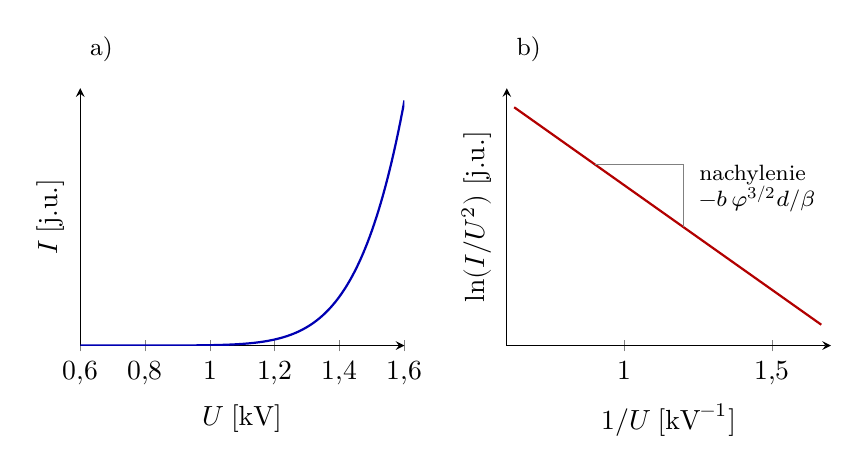
\begin{tikzpicture}
    \begin{axis}[name=iu,
        width=0.47\linewidth, height=0.40\linewidth,
        xmin=0.6, xmax=1.6, ymin=0, ymax=1.05,
        xlabel={$U$ [\si{\kilo\volt}]}, ylabel={$I$ [j.u.]},
        ytick=\empty, axis lines=left,
        title={a)}, title style={at={(0,1)}, anchor=south west, font=\small}]
      \addplot[thick, blue!70!black, domain=0.6:1.6, samples=150]
        {x^2*exp(-15/x)/(2.56*exp(-15/1.6))};
    \end{axis}
    \begin{axis}[at={($(iu.east)+(1.3cm,0)$)}, anchor=west,
        width=0.47\linewidth, height=0.40\linewidth,
        xmin=0.6, xmax=1.7, ymin=-26.5, ymax=-8,
        xlabel={$1/U$ [\si{\per\kilo\volt}]}, ylabel={$\ln(I/U^2)$ [j.u.]},
        ytick=\empty, axis lines=left,
        title={b)}, title style={at={(0,1)}, anchor=south west, font=\small}]
      \addplot[thick, red!70!black, domain=0.625:1.667, samples=2] {-15*x};
      \draw[gray] (axis cs:0.9,-13.5) -- (axis cs:1.2,-13.5) -- (axis cs:1.2,-18);
      \node[font=\footnotesize, anchor=west, align=left] at (axis cs:1.22,-15.2)
        {nachylenie\\$-b\,\varphi^{3/2}d/\beta$};
    \end{axis}
  \end{tikzpicture}
  \caption{Charakterystyka emisji polowej według równania Fowlera--Nordheima:
    a)~prąd emisji w~funkcji napięcia, b)~ta sama zależność we współrzędnych
    F--N \opracowanieWlasne}
  \label{fig:fn}
\end{figure}

Nanorurki węglowe (CNT) to zwinięte warstwy grafenu o~średnicy od ok.
\SI{1}{\nano\metre} (jednościenne) do kilkudziesięciu nanometrów
(wielościenne) i~długości do wielu mikrometrów. Jako emitery mają
kilka zalet~\cite{deheer1995cnt,milne2004cnt}:
\begin{itemize}
  \item bardzo duży stosunek długości do średnicy, a~więc duży
        współczynnik $\beta$ i~niskie napięcie progowe emisji,
  \item dobre przewodnictwo elektryczne i~cieplne,
  \item odporność chemiczną i~mechaniczną wiązań C--C, która ogranicza
        degradację wierzchołka,
  \item możliwość emisji z~wielu nanorurek jednocześnie, co daje duży
        prąd całkowity.
\end{itemize}
Pierwsze źródło elektronów z~CNT opisali de~Heer i~in. w~1995~r.
\cite{deheer1995cnt}, a~pierwsze lampy rentgenowskie z~katodą CNT
pojawiły się na początku XXI wieku
\cite{yue2002cntxray,heo2012miniature,parmee2015cntxray}. Katody CNT są
też rozważane w~układach napędu kosmicznego~\cite{huo2020cntspace}.

\subsection{Wywołanie emisji w~badanym układzie i~jej stabilność}

W~badanym układzie emisję wywołuje napięcie $U_\mathrm{B}$ przyłożone
między emiter (E) a~bramkę (B), czyli elektrodę ekstrakcyjną
z~otworem. Poniżej pewnego napięcia progowego prąd emisji jest
niemierzalny. Powyżej progu prąd rośnie wykładniczo zgodnie
z~\eqref{eq:fn}. Część elektronów trafia w~bramkę, a~część przechodzi
przez otwór i~jest przyspieszana w~stronę targetu (T) napięciem
$U_\mathrm{T}$. Sposób pomiaru prądów opisano w~\rozdzref{ch:stanowisko}.

Prąd emisji polowej jest wrażliwy na stan powierzchni emitera.
Cząsteczki gazu zaadsorbowane na wierzchołku zmieniają lokalną pracę
wyjścia, co powoduje fluktuacje prądu. Elektrony jonizują gaz resztkowy,
a~powstałe jony dodatnie są przyspieszane w~stronę emitera i~bombardują
go, co może uszkadzać nanorurki. Przy dużych prądach wierzchołki
nanorurek nagrzewają się i~mogą ulec przepaleniu. Dlatego źródło
odgazowuje się przez wygrzewanie, a~pomiary prowadzi przy możliwie
niskim ciśnieniu. Wpływ odgazowania na wyniki pomiarów omówiono
w~\pref{sec:emisja-magnes}.

% =====================================================================
\section{Przyspieszanie i~ogniskowanie wiązki elektronów}
\label{sec:wiazka}

\subsection{Energia elektronów i~napięcia w~układzie}

Elektron przyspieszany różnicą potencjałów $U$ uzyskuje energię
kinetyczną
\begin{equation}
  E = eU,
\end{equation}
czyli np. \SI{10}{\kilo\electronvolt} przy \SI{10}{\kilo\volt}. Prędkość
elektronu wynosi $v=\sqrt{2eU/m_\mathrm{e}}$, co dla \SI{10}{\kilo\volt} daje
ok. \SI{5.9e7}{\metre\per\second}.

W~układzie występują dwa napięcia o~różnych funkcjach:
\begin{itemize}
  \item \textbf{napięcie ekstrakcyjne} $U_\mathrm{B}$ (emiter--bramka)
        -- decyduje o~natężeniu pola na emiterze, a~więc o~prądzie emisji,
  \item \textbf{napięcie przyspieszające} $U_\mathrm{T}$ (emiter--target)
        -- decyduje o~energii elektronów padających na target lub próbkę,
        a~więc o~tym, które linie charakterystyczne mogą zostać wzbudzone
        (p.~\ref{subsec:jonizacja}).
\end{itemize}
Rozdzielenie tych funkcji pozwala regulować prąd wiązki niezależnie od
jej energii. Wartości napięć stosowanych w~badaniach podano
w~\rozdzref{ch:stanowisko}.

Aby elektrony były przyspieszane w~kierunku targetu, target musi mieć
potencjał dodatni względem emitera. Można to uzyskać na dwa sposoby:
uziemić emiter i~doprowadzić do targetu napięcie $+U_\mathrm{T}$ albo
uziemić target i~spolaryzować emiter napięciem $-U_\mathrm{T}$. Drugi
sposób jest prostszy w~realizacji: próbka, uchwyt i~komora pozostają na
potencjale masy, więc między próbką a~detektorem i~ściankami komory nie
występuje pole odchylające elektrony ani ryzyko przebicia do detektora,
a~wysokie napięcie jest doprowadzone tylko do niewielkiego emitera.
Wymaga on jednak zasilacza wysokiego napięcia o~ujemnej polaryzacji
wyjścia, a~obwód bramki musi być wtedy odniesiony do potencjału emitera.
W~badaniach prototypu zastosowano pierwszy sposób, z~dodatnim napięciem
$U_\mathrm{T}$ doprowadzonym do targetu (\rozdzref{ch:stanowisko}).

\subsection{Ruch elektronu i~ogniskowanie w~polu magnetycznym}

Na elektron poruszający się w~polu elektrycznym $\vec{E}$ i~magnetycznym
$\vec{B}$ działa siła Lorentza
\begin{equation}
  \vec{F} = -e\left(\vec{E} + \vec{v}\times\vec{B}\right).
\end{equation}
Składowa prędkości równoległa do linii pola magnetycznego nie zmienia
się, a~składowa prostopadła $v_\perp$ powoduje ruch po okręgu
o~promieniu Larmora
\begin{equation}
  r_\mathrm{L} = \frac{m_\mathrm{e} v_\perp}{eB}.
\end{equation}
Wypadkowy ruch to spirala nawinięta na linię pola. Elektrony wylatujące
z~emitera pod różnymi kątami są więc utrzymywane w~pobliżu linii pola
przechodzących przez emiter, zamiast rozbiegać się na boki. Przy indukcji
rzędu \SI{0.1}{\tesla} i~składowej poprzecznej energii rzędu
\SI{10}{\electronvolt} promień Larmora wynosi ok.
\SI{0.1}{\milli\metre}.

Pole magnetyczne o~symetrii osiowej działa na wiązkę elektronów jak
soczewka skupiająca. W~przybliżeniu cienkiej soczewki jej ogniskową
opisuje wzór Buscha
\begin{equation}
  \frac{1}{f} = \frac{e}{8 m_\mathrm{e} U}\int B_z^2(z)\,\mathrm{d}z,
\end{equation}
z~którego wynika, że ogniskowanie jest tym silniejsze, im większa jest
indukcja i~im mniejsza energia elektronów~\cite{goldstein2018sem}.
W~mikroskopach elektronowych stosuje się elektromagnesy z~nabiegunnikami.
W~miniaturowym źródle MEMS, podobnie jak w~badanym prototypie, stosuje
się prosty magnes trwały NdFeB umieszczony pod emiterem. Elektrony
podążają wzdłuż jego linii pola, co poprawia skupienie i~jednorodność
wiązki w~porównaniu z~samym ogniskowaniem
elektrostatycznym~\cite{urbanski2026phd,grzebyk2017magnetic}.

\subsection{Ogniskowanie elektrostatyczne i~obserwacja wiązki}

Wiązkę można też ogniskować polem elektrycznym elektrod o~odpowiednio
ukształtowanych otworach (soczewki elektrostatyczne, np. pojedyncza
soczewka Einzela). W~strukturach MEMS elektrody takie wykonuje się
z~krzemu, ale ich wymiary i~odległości są ograniczone grubością płytek,
a~ich ustawienie względem siebie musi być bardzo dokładne. W~pracy
\cite{urbanski2026phd} samo ogniskowanie elektrostatyczne okazało się
niewystarczające, co uzasadnia użycie magnesu.

Kształt i~położenie wiązki obserwuje się na ekranie pokrytym luminoforem,
który świeci w~miejscu padania elektronów. Jasność świecenia rośnie
z~gęstością prądu, dlatego zdjęcie ekranu pokazuje rozkład gęstości
prądu w~przekroju wiązki. Metoda ta jest jakościowa: jasność zależy też
od energii elektronów, rodzaju luminoforu, jego degradacji i~ustawień
aparatu.

% =====================================================================
\section{Powstawanie promieniowania X}
\label{sec:rtg}

\subsection{Oddziaływanie elektronów z~materią i~promieniowanie hamowania}

Elektron wnikający w~materiał ulega rozpraszaniu sprężystemu (na
jądrach, zmiana kierunku bez straty energii) i~niesprężystemu (na
elektronach atomów, strata energii). Wypadkowa trajektoria jest
zygzakowata, a~obszar, w~którym zachodzą oddziaływania, ma kształt
gruszki lub półkuli pod punktem padania wiązki. Produktami oddziaływań
są elektrony wtórne, elektrony wstecznie rozproszone, ciepło oraz
promieniowanie X: ciągłe i~charakterystyczne~\cite{goldstein2018sem}.

Głębokość wnikania elektronów opisuje zasięg Kanayi--Okayamy
\begin{equation}
  R\,[\si{\micro\metre}] = \frac{0{,}0276\,A\,E_0^{1{,}67}}{Z^{0{,}89}\,\rho},
\end{equation}
gdzie $A$ -- masa atomowa [g/mol], $E_0$ -- energia elektronów [keV],
$Z$ -- liczba atomowa, $\rho$ -- gęstość [g/cm$^3$]. Dla krzemu zasięg
wynosi ok. \SI{1.5}{\micro\metre} przy \SI{10}{\kilo\electronvolt}
i~ok. \SI{0.3}{\micro\metre} przy \SI{4}{\kilo\electronvolt}.
Analiza EDS dotyczy więc warstwy przypowierzchniowej próbki o~grubości
rzędu mikrometrów.

Elektron hamowany w~polu elektrycznym jądra traci część energii, która
jest emitowana jako foton. Ponieważ strata energii w~pojedynczym
zdarzeniu może mieć dowolną wartość od zera do całej energii elektronu,
widmo promieniowania hamowania (\emph{bremsstrahlung}) jest ciągłe.
Kształt widma opisuje w~przybliżeniu wzór Kramersa
\begin{equation}
  N(E) \approx k\,i\,Z\,\frac{E_0-E}{E},
\end{equation}
gdzie $N(E)$ jest liczbą fotonów o~energii $E$ w~jednostkowym przedziale
energii, $i$ -- prądem wiązki, $k$ -- stałą. Widmo kończy się na
energii równej energii elektronów (granica Duane'a--Hunta):
\begin{equation}
  E_\mathrm{max} = eU, \qquad
  \lambda_\mathrm{min}\,[\si{\nano\metre}] = \frac{1{,}2398}{U\,[\si{\kilo\volt}]}.
\end{equation}
W~analizie EDS promieniowanie hamowania stanowi tło, na którym widoczne
są linie charakterystyczne. Pomiar granicy Duane'a--Hunta w~widmie pozwala
sprawdzić rzeczywistą energię elektronów docierających do próbki. Kształt widma dla dwóch energii elektronów przedstawiono na
rys.~\ref{fig:kramers}.

\begin{figure}[htbp]
  \centering
  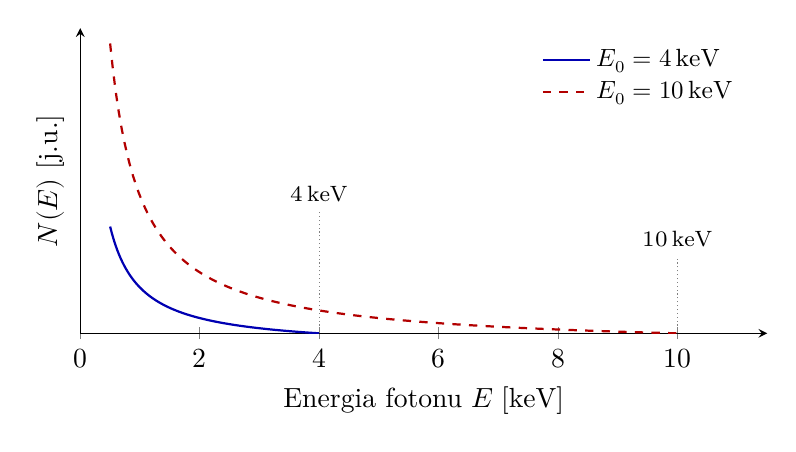
\begin{tikzpicture}
    \begin{axis}[
        width=0.85\linewidth, height=0.45\linewidth,
        xmin=0, xmax=11.5, ymin=0, ymax=20,
        xlabel={Energia fotonu $E$ [\si{\kilo\electronvolt}]},
        ylabel={$N(E)$ [j.u.]},
        ytick=\empty, axis lines=left,
        legend style={draw=none, font=\small}, legend cell align=left, legend pos=north east]
      \addplot[thick, blue!70!black, domain=0.5:4, samples=120]
        {(4-x)/x};
      \addlegendentry{$E_0=\SI{4}{\kilo\electronvolt}$}
      \addplot[thick, red!70!black, dashed, domain=0.5:10, samples=200]
        {(10-x)/x};
      \addlegendentry{$E_0=\SI{10}{\kilo\electronvolt}$}
      \draw[gray, densely dotted] (axis cs:4,0) -- (axis cs:4,8)
        node[above, font=\footnotesize, black] {\SI{4}{\kilo\electronvolt}};
      \draw[gray, densely dotted] (axis cs:10,0) -- (axis cs:10,5)
        node[above, font=\footnotesize, black] {\SI{10}{\kilo\electronvolt}};
    \end{axis}
  \end{tikzpicture}
  \caption{Widmo promieniowania hamowania według wzoru Kramersa dla
    energii elektronów stosowanych w~badaniach (\SI{4}{} i~\SI{10}{\kilo\electronvolt});
    widmo kończy się na granicy Duane'a--Hunta
    $E_\mathrm{max}=eU$. Na widmo ciągłe nakładają się linie
    charakterystyczne, a~przy małych energiach jest ono osłabiane przez
    absorpcję w~próbce i~oknie detektora \opracowanieWlasne}
  \label{fig:kramers}
\end{figure}

\subsection{Jonizacja powłok wewnętrznych}
\label{subsec:jonizacja}

Elektron wiązki może wybić elektron z~wewnętrznej powłoki atomu (K, L,
M), jeśli jego energia jest większa od energii wiązania tej powłoki,
nazywanej energią krytyczną $E_\mathrm{c}$ (odpowiada ona krawędzi
absorpcji). Na przykład dla powłoki K krzemu
$E_\mathrm{c}=\SI{1.84}{\kilo\electronvolt}$, a~dla żelaza
\SI{7.11}{\kilo\electronvolt}. Stosunek energii elektronów do energii
krytycznej nazywa się współczynnikiem nadnapięcia
\begin{equation}
  U_0 = \frac{E_0}{E_\mathrm{c}}.
\end{equation}
Natężenie linii charakterystycznej rośnie w~przybliżeniu jak
$(U_0-1)^{n}$, gdzie $n\approx1{,}5$--$1{,}7$. W~praktyce do skutecznego
wzbudzenia linii stosuje się $U_0\approx2$--3. Przy energii
\SI{4}{\kilo\electronvolt} warunek $U_0\geq2$ spełniają linie K
pierwiastków o~energii krytycznej do ok. \SI{2}{\kilo\electronvolt}
(O, Na, Mg, Al, Si), a~linii K wapnia ($E_\mathrm{c}=\SI{4.04}{\kilo\electronvolt}$)
i~cięższych pierwiastków nie da się wzbudzić. Przy \SI{10}{\kilo\electronvolt}
dobrze wzbudzane są linie K pierwiastków do ok. tytanu, a~linie K żelaza
($U_0\approx1{,}4$) i~miedzi ($U_0\approx1{,}1$) już słabo. Metale
przejściowe i~pierwiastki ciężkie rozpoznaje się wtedy głównie po liniach
L i~M (np. Cu L$\alpha$ \SI{0.930}{\kilo\electronvolt}). Skuteczne
wzbudzenie linii K głównych pierwiastków skałotwórczych łącznie
z~żelazem ($U_0 \geq 2$) wymaga energii ok.~\SI{15}{\kilo\electronvolt},
co uzasadnia docelowe napięcie przyspieszające do ok.~\SI{18}{\kilo\volt}.

\subsection{Relaksacja atomu, nazewnictwo linii i~prawo Moseleya}

Po jonizacji powłoki wewnętrznej atom znajduje się w~stanie wzbudzonym.
Lukę zapełnia elektron z~wyższej powłoki, a~nadmiar energii, równy
różnicy energii wiązania obu powłok, zostaje wypromieniowany jako foton
promieniowania X. Energie powłok są inne dla każdego pierwiastka, dlatego
energia fotonu jest cechą charakterystyczną pierwiastka i~na niej opiera
się identyfikacja składu w~spektroskopii EDS. Przykładowo przejście
elektronu z~powłoki L na powłokę K w~atomie glinu daje foton Al~\Ka{}
o~energii \SI{1.487}{\kilo\electronvolt}.

Nie każda relaksacja kończy się emisją fotonu. W~konkurencyjnym efekcie
Augera nadmiar energii przejmuje inny elektron atomu, który opuszcza atom,
i~foton nie powstaje. Udział relaksacji z~emisją fotonu opisuje wydajność
fluorescencji $\omega$, rosnąca z~liczbą atomową: dla powłoki K krzemu
wynosi ok.~\num{0.05}, a~dla żelaza ok.~\num{0.35}. Lekkie pierwiastki
emitują więc mniej fotonów na jedną jonizację i~dają w~widmie słabsze
linie~\cite{goldstein2018sem,beckhoff2006xrf}.

Linie oznacza się literą powłoki, na której powstała luka, oraz
indeksem określającym, skąd pochodzi elektron zapełniający:
K$\alpha$ (przejście L$\to$K), K$\beta$ (M$\to$K), L$\alpha$ (M$\to$L)
itd. (notacja Siegbahna; w~notacji IUPAC np. K$\alpha_1$ = K--L$_3$).
Energia linii zależy od liczby atomowej zgodnie z~prawem Moseleya.
Dla linii K$\alpha$ w~przybliżeniu
\begin{equation}
  E_{\mathrm{K}\alpha} \approx \SI{10.2}{\electronvolt}\,(Z-1)^2,
\end{equation}
co np. dla żelaza ($Z=26$) daje ok. \SI{6.4}{\kilo\electronvolt},
zgodnie z~wartością tablicową. Jednoznaczna zależność energii linii od
$Z$ jest podstawą identyfikacji pierwiastków w~widmie.
Przykładowe energie linii K$\alpha$: O~\SI{0.525}{\kilo\electronvolt},
Mg \SI{1.254}{\kilo\electronvolt}, Al \SI{1.487}{\kilo\electronvolt},
Si \SI{1.740}{\kilo\electronvolt}, Ca \SI{3.69}{\kilo\electronvolt},
Fe \SI{6.40}{\kilo\electronvolt}.

\subsection{EDS a~XRF}

Obie metody rejestrują to samo promieniowanie charakterystyczne, ale
różnią się sposobem wzbudzenia:
\begin{itemize}
  \item w~\textbf{EDS} (w~mikroskopie elektronowym) próbkę wzbudza wiązka
        elektronów. Wiązkę łatwo zogniskować do małej plamki
        i~wydajnie wzbudza ona pierwiastki lekkie, ale towarzyszy jej
        silne tło promieniowania hamowania, a~próbka nieprzewodząca może
        się ładować;
  \item w~\textbf{XRF} próbkę wzbudzają fotony promieniowania X (z~lampy
        rentgenowskiej lub izotopu). Tło jest znacznie mniejsze, bo nie
        powstaje promieniowanie hamowania w~próbce, ale wzbudzenie
        pierwiastków lekkich jest słabsze, a~ogniskowanie promieniowania
        X wymaga specjalnej optyki~\cite{beckhoff2006xrf}.
\end{itemize}
Miniaturowe źródło RTG MEMS rozwijane na Politechnice Wrocławskiej
zastosowano dotychczas do spektrometrii XRF~\cite{urbanski2026xrf}.
W~tej pracy wiązka elektronów pada bezpośrednio na próbkę, czyli
przyrząd działa jak analizator EDS.

\subsection{Target transmisyjny i~odbiciowy}
\label{subsec:target}

W~źródle rentgenowskim MEMS wiązka elektronów pada na target
transmisyjny: cienką warstwę metalu na membranie, przez którą
promieniowanie wychodzi wzdłuż osi wiązki~\cite{urbanski2023target,urbanski2024monochromatic}.
W~analizatorze EDS opisanym w~tej pracy membrany nie ma, a~wiązka
elektronów pada bezpośrednio na badaną próbkę (\pref{sec:koncepcja}).

% =====================================================================
\section{Pomiar widma metodą EDS}
\label{sec:spektrometria}

\subsection{Półprzewodnikowy detektor promieniowania X}

Foton promieniowania X pochłonięty w~krysztale półprzewodnika wytwarza
pary elektron--dziura. Średnia energia na wytworzenie jednej pary
w~krzemie wynosi $\varepsilon\approx\SI{3.6}{\electronvolt}$, więc foton
o~energii \SI{6}{\kilo\electronvolt} wytwarza ok.~\num{1600} par. Pole
elektryczne w~detektorze rozdziela nośniki, zanim zdążą zrekombinować,
i~zbiera je na elektrodach. Zebrany ładunek jest proporcjonalny do
energii fotonu~\cite{urbanski2023detection}.

Stosowane typy detektorów:
\begin{itemize}
  \item \textbf{Si(Li)} -- krzem kompensowany litem, wymaga chłodzenia
        ciekłym azotem,
  \item \textbf{SDD} (krzemowy detektor dryfowy) -- elektrony dryfują do
        małej anody o~niskiej pojemności, co obniża szumy i~pozwala na
        duże szybkości zliczeń. Chłodzony ogniwem Peltiera, obecnie
        najczęściej stosowany,
  \item \textbf{CdTe} -- wyższa liczba atomowa, lepsza wydajność dla
        energii powyżej ok. \SI{20}{\kilo\electronvolt}, gorsza
        rozdzielczość.
\end{itemize}
Typu detektora w~spektrometrze użytym do pomiarów nie ustalono, dlatego
zasadę działania opisano ogólnie.

\subsection{Tor akwizycji i~analiza widma}

Ładunek z~detektora jest zamieniany na impuls napięciowy przez
przedwzmacniacz ładunkowy. Układ kształtujący (obecnie cyfrowy procesor
impulsów) filtruje sygnał i~mierzy amplitudę każdego impulsu.
Analizator wielokanałowy (MCA) przypisuje impuls do kanału odpowiadającego
jego amplitudzie i~zlicza impulsy w~kanałach. Wynikiem jest histogram
liczby zliczeń w~funkcji energii, czyli widmo.

Analiza jakościowa polega na przypisaniu pikom pierwiastków na
podstawie energii linii. Należy uwzględnić zjawiska, które dają piki
pozorne lub zniekształcenia:
\begin{itemize}
  \item \textbf{tło promieniowania hamowania}, które trzeba odjąć przed
        wyznaczeniem pola powierzchni pików,
  \item \textbf{piki ucieczki} -- foton padający wzbudza w~detektorze
        krzemowym promieniowanie Si K$\alpha$, które ucieka z~kryształu.
        Rejestrowana jest wtedy energia mniejsza o~\SI{1.74}{\kilo\electronvolt},
  \item \textbf{piki sumacyjne} -- dwa fotony zarejestrowane niemal
        jednocześnie dają impuls o~sumie ich energii,
  \item \textbf{nakładanie się linii} różnych pierwiastków o~zbliżonych
        energiach (np. S K$\alpha$ \SI{2.31}{\kilo\electronvolt}
        i~Mo L$\alpha$ \SI{2.29}{\kilo\electronvolt}),
  \item \textbf{linie pochodzące z~elementów konstrukcji} (bramka,
        uchwyt, ścianki komory), w~które trafiają elektrony rozproszone.
\end{itemize}

Oprócz spektroskopii z~dyspersją energii (EDS) stosuje się spektroskopię
z~dyspersją długości fali (WDS), w~której promieniowanie jest
rozszczepiane przez odbicie od kryształu analizatora (warunek Bragga).
WDS ma rozdzielczość rzędu \SI{10}{\electronvolt}, ale wymaga ruchomego
goniometru, rejestruje naraz jedną linię i~jest duży. EDS rejestruje całe
widmo jednocześnie w~małym detektorze bez części ruchomych, dlatego
nadaje się do miniaturowego przyrządu kosmicznego~\cite{goldstein2018sem}.

\subsection{Analiza ilościowa i~niepewność pomiaru}

Skład ilościowy wyznacza się z~natężeń linii, porównując je z~natężeniami
zmierzonymi dla wzorców o~znanym składzie. Wymaga to poprawek na liczbę
atomową, absorpcję i~fluorescencję wtórną w~próbce (poprawki ZAF) oraz
płaskiej, wypolerowanej powierzchni próbki i~stabilnego prądu wiązki.
W~tej pracy prąd wiązki i~geometria pomiaru nie były na tyle stabilne
i~znane, aby prowadzić analizę ilościową, dlatego ograniczono się do
analizy jakościowej.

Zliczenia fotonów podlegają rozkładowi Poissona, więc niepewność liczby
zliczeń $N$ w~piku wynosi $\sqrt{N}$, a~niepewność względna $1/\sqrt{N}$.
Do uzyskania niepewności względnej \SI{1}{\percent} potrzeba ok.
\num{10000} zliczeń w~piku. Niepewność pomiaru prądu wynika z~klasy
woltomierza i~tolerancji rezystora (\SI{100}{\kilo\ohm}), a~niepewność
napięć z~dokładności zasilaczy.

% =====================================================================
\section{Próżnia i~warunki pracy przyrządu}
\label{sec:uzupelnienia}

\subsection{Próżnia}

Elektrony muszą przebyć drogę od emitera do próbki bez zderzeń
z~cząsteczkami gazu. Średnia droga swobodna cząsteczki powietrza
w~temperaturze pokojowej wynosi w~przybliżeniu
$\bar l\,[\si{\milli\metre}] \approx 6{,}6/p\,[\si{\pascal}]$,
a~dla elektronu jest ok. 5--6 razy większa. Przy ciśnieniu
\SI{1e-5}{\milli\bar} (\SI{1e-3}{\pascal}) droga swobodna elektronu
wynosi kilkadziesiąt metrów, czyli wielokrotnie więcej niż wymiary
struktury. Niskie ciśnienie jest potrzebne także ze względu na trwałość
emitera (bombardowanie jonowe, adsorpcja gazów) i~ryzyko wyładowań między
elektrodami.

W~docelowej strukturze hermetycznej (p.~\ref{subsec:bonding}) próżnię
podtrzymywałaby zintegrowana mikropompa jonowo-sorpcyjna. Wiązka
elektronów wywołuje desorpcję gazów ze ścianek (desorpcja stymulowana
elektronami), więc sama hermetyzacja nie wystarcza do utrzymania próżni
\cite{grzebyk2014micropump,grzebyk2017pumps,urbanski2026phd}.

\subsection{Warunki pracy w~misji kosmicznej}
\label{subsec:warunki}

Naturalna próżnia na powierzchni Księżyca (rzędu \SI{1e-10}{\pascal})
i~planetoid wystarcza do propagacji wiązki elektronów. Na Marsie ciśnienie atmosfery CO$_2$
wynosi ok. \SI{600}{\pascal}, więc wiązka elektronów musiałaby przejść
przez cienkie okno lub krótki odcinek gazu. Rozwiązania tego typu
rozważano dla miniaturowych mikroskopów ze zmiennym ciśnieniem
\cite{gaskin2012mvpsem,thaisen2010minisem}.
Przyrząd musi ponadto znosić promieniowanie kosmiczne, duże zmiany
temperatury i~przeciążenia przy starcie, a~jego masa i~pobór mocy są
ograniczone budżetem misji. Przyrządy stosowane dotąd w~misjach
(APXS, PIXL) wzbudzają próbkę cząstkami alfa lub promieniowaniem~X
(\rozdzref{ch:wstep}).

\subsection{Zasilanie i~sterowanie}

Źródło wymaga dwóch napięć: ekstrakcyjnego (rzędu \SI{1}{\kilo\volt})
i~przyspieszającego (docelowo \SIrange{10}{18}{\kilo\volt}). W~przyrządach
przenośnych i~kosmicznych wysokie napięcie uzyskuje się z~przetwornicy
z~transformatorem podwyższającym i~powielaczem napięcia
Cockcrofta--Waltona. Ponieważ prąd emisji polowej zmienia się
wykładniczo z~napięciem i~zależy od stanu powierzchni emitera,
w~docelowym przyrządzie potrzebna jest pętla sprzężenia zwrotnego, która
mierzy prąd wiązki i~koryguje napięcie ekstrakcyjne. Utrzymuje to stałą
częstość zliczeń w~widmie i~chroni emiter przed przeciążeniem.

        % 9. wprowadzenie teoretyczne
% Rozdział 3 — Projekt i wykonanie prototypu (budżet: 6,5 str.)
% Źródło: projekt-prototypu/projekt.tex (ma własne \chapter i \label{ch:projekt}).
% Plan akapitów i brakujące dane (T1–T20): wspolne/rozdzial3_plan.md
% =====================================================================
%  Rozdział 3 — Projekt i wykonanie prototypu (budżet: 6,5 str., ok. 1500 słów)
%  Plan akapitów: wspolne/rozdzial3_plan.md (oznaczenia T1–T20 = brakujące dane)
%  17.11.2026 (przegląd spójności): puste podrozdziały 3.3–3.5 (projekt
%  elektrod, maski, wytwarzanie Si) scalono z p. „Przebieg wytwarzania
%  struktury”; ich brakujące dane (T6–T14) zebrano w jednym \TODO tam.
%  Zamknięte z treści pracy: T1 (magnes pod emiterem), T2 (różnice wobec
%  źródła RTG opisane w akapicie), T5 częściowo i T8 (drugie szkło 1 mm,
%  elektroda skupiająca z Si).
% =====================================================================
\chapter{Projekt i~wykonanie prototypu}
\label{ch:projekt}

Na podstawie zasad przedstawionych w~\rozdzref{ch:podstawy} opracowano
i~wykonano prototyp źródła elektronów analizatora. W~rozdziale opisano projekt struktury krzemowo-szklanej źródła elektronów
oraz kolejne etapy jej wytworzenia, aż do zmontowanego prototypu. Zasady
zastosowanych procesów technologicznych omówiono w~\pref{sec:technologia}.

% ---------------------------------------------------------------------
\section{Założenia projektowe i~koncepcja struktury}
\label{sec:koncepcja}

Prototyp miał spełniać następujące wymagania:
\begin{itemize}[nosep]
  \item wytworzenie wiązki elektronów przez emisję polową z~nanorurek
        węglowych przy napięciu ekstrakcyjnym $\UB$ rzędu \SI{1}{\kilo\volt},
  \item przyspieszenie elektronów do energii wystarczającej do wzbudzenia
        linii charakterystycznych pierwiastków lekkich (w~badaniach
        $\UT$ do \SI{10}{\kilo\volt}, docelowo do \SI{18}{\kilo\volt}),
  \item izolacja elektryczna elektrod przy tych napięciach,
  \item wykonanie wyłącznie procesami MEMS: fotolitografią, trawieniem
        krzemu i~bondingiem anodowym krzem--szkło,
  \item możliwość późniejszej hermetyzacji struktury.
\end{itemize}

Strukturę zaprojektowano jako stos płaskich elementów krzemowych
rozdzielonych szkłem borokrzemowym (\rysref{fig:przekroj-struktury}).
Licząc od dołu, składa się ona z~emitera (E) z~ostrzem uformowanym
z~nanorurek węglowych, szkła dystansowego o~grubości \SI{1}{\milli\metre},
bramki (elektrody ekstrakcyjnej, B), drugiego szkła dystansowego oraz
elektrody skupiającej z~otworem (T, w~dalszej części pracy nazywanej
targetem). Każda elektroda krzemowa jest osobnym elementem
z~własnym kontaktem elektrycznym, a~szkło oddziela je galwanicznie
i~ustala odległości między nimi. Wiązkę ogniskuje magnes trwały NdFeB
umieszczony pod emiterem.

\begin{figure}[htbp]
  \centering
  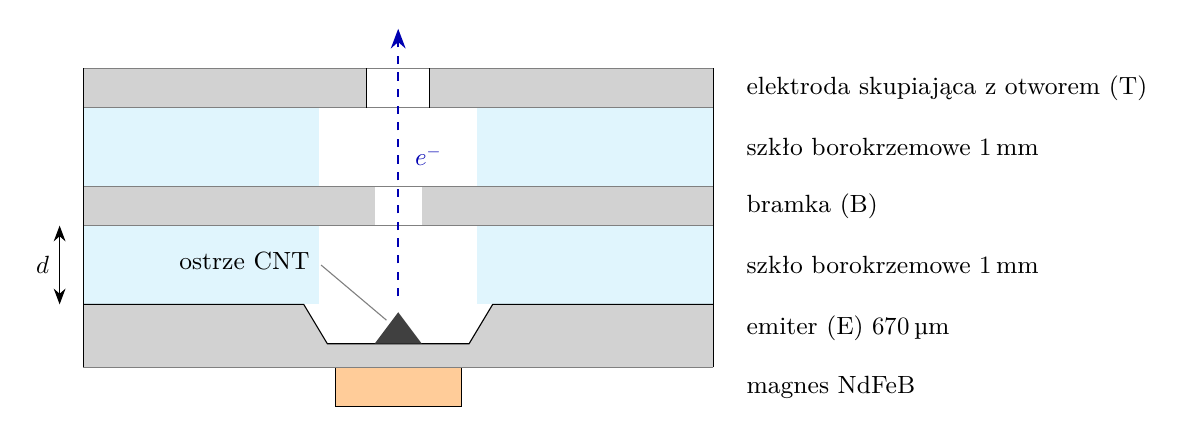
\begin{tikzpicture}[x=1cm, y=1cm, font=\small]
    % kolory
    \colorlet{si}{gray!35}
    \colorlet{gl}{cyan!12}
    % elektroda skupiająca z otworem
    \fill[si] (0,4.4) rectangle (3.6,4.9);
    \fill[si] (4.4,4.4) rectangle (8,4.9);
    % szkło 2 z otworem
    \fill[gl] (0,3.4) rectangle (3,4.4);
    \fill[gl] (5,3.4) rectangle (8,4.4);
    % bramka z aperturą
    \fill[si] (0,2.9) rectangle (3.7,3.4);
    \fill[si] (4.3,2.9) rectangle (8,3.4);
    % szkło 1 z otworem
    \fill[gl] (0,1.9) rectangle (3,2.9);
    \fill[gl] (5,1.9) rectangle (8,2.9);
    % emiter: wnęka od góry, pocienione dno
    \fill[si] (0,1.1) -- (8,1.1) -- (8,1.9) -- (5.2,1.9) -- (4.9,1.4)
      -- (3.1,1.4) -- (2.8,1.9) -- (0,1.9) -- cycle;
    \draw (0,1.9) -- (2.8,1.9) -- (3.1,1.4) -- (4.9,1.4) -- (5.2,1.9) -- (8,1.9);
    % ostrze (wieża) CNT na dnie wnęki
    \fill[black!75] (3.7,1.4) -- (4,1.8) -- (4.3,1.4) -- cycle;
    % magnes pod emiterem
    \fill[orange!40] (3.2,0.6) rectangle (4.8,1.1);
    \draw (3.2,0.6) rectangle (4.8,1.1);
    % obrysy
    \foreach \y in {1.1,2.9,3.4,4.4,4.9} {\draw[gray] (0,\y) -- (8,\y);}
    \draw (0,1.1) -- (0,4.9) (8,1.1) -- (8,4.9);
    \draw (3.6,4.4) -- (3.6,4.9) (4.4,4.4) -- (4.4,4.9);
    % wiązka
    \draw[-{Stealth[length=2.5mm]}, blue!70!black, thick, dashed]
      (4,2.0) -- (4,5.4);
    % opisy
    \foreach \y/\t in {4.65/elektroda skupiająca z~otworem (T),
                       3.9/szkło borokrzemowe \SI{1}{\milli\metre},
                       3.15/bramka (B),
                       2.4/szkło borokrzemowe \SI{1}{\milli\metre},
                       1.6/emiter (E) \SI{670}{\micro\metre},
                       0.85/magnes NdFeB}
      {\node[anchor=west] at (8.3,\y) {\t};}
    \node[anchor=east] at (3.0,2.45) {ostrze CNT};
    \draw[gray] (3.02,2.4) -- (3.85,1.7);
    \node[anchor=west, blue!70!black] at (4.1,3.75) {$e^-$};
    % wymiar
    \draw[{Stealth[length=2mm]}-{Stealth[length=2mm]}] (-0.3,1.9) -- (-0.3,2.9)
      node[midway, left] {$d$};
  \end{tikzpicture}
  \caption{Przekrój struktury prototypu (schemat poglądowy, bez zachowania
    skali): E -- emiter z~wnęką, na której dnie znajduje się
    ostrze CNT, B -- bramka (elektroda ekstrakcyjna), T -- elektroda skupiająca
    z~otworem; $d$ -- odległość emiter--bramka
    \opracowanieWlasne}
  \label{fig:przekroj-struktury}
\end{figure}

W~porównaniu ze źródłem promieniowania rentgenowskiego opisanym
w~\cite{urbanski2026phd} konstrukcja jest uproszczona: nie ma
zintegrowanej mikropompy ani targetu transmisyjnego z~membraną krzemową.
Zamiast membrany górnym elementem struktury jest elektroda skupiająca
z~otworem, przez który wiązka wychodzi ze struktury i~pada bezpośrednio
na próbkę (lub warstwę luminoforu).
Sposób zasilania elektrod opisano w~\rozdzref{ch:stanowisko}.

% ---------------------------------------------------------------------
\section{Dobór materiałów i~grubości elementów}
\label{sec:materialy}

Elektrody wykonano z~płytek krzemu monokrystalicznego o~orientacji
(100), ponieważ kształt otworów uzyskuje się trawieniem
anizotropowym (\pref{subsec:koh}), a~krzem jest jednocześnie materiałem
konstrukcyjnym i~przewodzącym. Emiter ma wymiary
\qtyproduct[product-units=single]{14 x 14}{\milli\metre} i~grubość \SI{670}{\micro\metre}; w~jego części środkowej, od strony bramki, wytrawiono
wnękę, na której dnie znajduje się ostrze CNT (\pref{sec:przebieg}).
\TODO{T4: grubość bramki i~elektrody skupiającej; typ i~rezystywność płytek Si}

Jako dystansownik między emiterem a~bramką zastosowano szkło
borokrzemowe o~grubości \SI{1}{\milli\metre}. Grubość szkła wyznacza
bezpośrednio odległość emiter--bramka $d$, a~więc natężenie pola
elektrycznego przy emiterze. Przy $d \approx \SI{1}{\milli\metre}$
i~$\UB = \SI{1}{\kilo\volt}$ średnie natężenie pola wynosi ok.
\SI{1}{\volt\per\micro\metre}; lokalne pole na wierzchołkach nanorurek
jest wielokrotnie większe dzięki współczynnikowi wzmocnienia pola
(\pref{sec:emisja}). Ostrze CNT o~wysokości ok.~\SI{360}{\micro\metre}
(\pref{sec:nanoszenie-cnt}) stoi na dnie wnęki o~głębokości
\SI{430}{\micro\metre} (\SI{670}{} $-$ \SI{240}{\micro\metre}), więc jego
wierzchołek leży ok.~\SI{70}{\micro\metre} poniżej górnej powierzchni
emitera, a~odległość wierzchołek--bramka wynosi ok.~$d + \SI{70}{\micro\metre}$.
Ostrze nie skraca więc odległości od bramki, lecz skupia pole na
wierzchołku i~wyprowadza go ponad dno wnęki.
\TODO{T7: średnica apertury bramki}

Drugim zadaniem szkła jest izolacja elektrod. W~próżni ograniczeniem
jest przede wszystkim przeskok wzdłuż powierzchni szkła między krawędziami
sąsiednich elektrod, dlatego grubość dystansownika wyznacza też drogę
upływu. Między bramką a~targetem występuje różnica potencjałów
$\UT - \UB$, a~między emiterem a~bramką $\UB$. Przy napięciach
stosowanych w~badaniach (do \SI{10}{\kilo\volt}) oba szkła o~grubości
\SI{1}{\milli\metre} zapewniały wystarczającą izolację. Przy napięciach
wyższych, docelowo do \SI{18}{\kilo\volt}, potrzebne są dodatkowe
zabezpieczenia, np. zalanie krawędzi struktury żywicą epoksydową, jak
w~\cite{urbanski2026phd}.
\TODO{T5: typ szkła (Borofloat~33?)}

Szkło borokrzemowe ma współczynnik rozszerzalności cieplnej zbliżony do
krzemu i~zawiera jony sodu, dzięki czemu można je łączyć z~krzemem
bondingiem anodowym (\pref{subsec:bonding}). Duża odległość między
emiterem a~targetem sprzyja jednak rozbieganiu się wiązki, co uzasadnia
zastosowanie magnesu ogniskującego (\pref{sec:wiazka}).
Wymiary wszystkich elementów zestawiono w~\tabref{tab:elementy-struktury}.

\begin{table}[htbp]
  \centering
  \caption{Elementy struktury prototypu (od dołu)}
  \label{tab:elementy-struktury}
  \begin{tabular}{@{}llll@{}}
    \toprule
    Element & Materiał & Grubość & Funkcja \\
    \midrule
    emiter (E)        & Si (100) + ostrze CNT & \SI{670}{\micro\metre} & źródło elektronów \\
    dystansownik      & szkło borokrzemowe   & \SI{1}{\milli\metre} & izolacja, odległość $d$ \\
    bramka (B)        & Si (100)             & \TODOtab{T4}           & elektroda ekstrakcyjna \\
    dystansownik      & szkło borokrzemowe   & \SI{1}{\milli\metre} & izolacja B--T \\
    elektroda skupiająca (T) & Si (100)      & \TODOtab{T4}           & wyjście wiązki przez otwór \\
    magnes ogniskujący & NdFeB (pod emiterem) & --                  & ogniskowanie wiązki \\
    \bottomrule
  \end{tabular}
\end{table}

\section{Przebieg wytwarzania struktury}
\label{sec:przebieg}

Kolejność czynności prowadzących do gotowej struktury przedstawiono na
\rysref{fig:proces}. Elementy krzemowe i~szklane wytwarzano równolegle
na całych płytkach, a~dopiero po ich pocięciu łączono je w~stos.
W~emiterze trawieniem w~KOH (\pref{subsec:koh}) wykonano wnękę od strony
bramki, pozostawiając dno o~grubości \SI{240}{\micro\metre}, na którym
formowano ostrze CNT. W~bramce i~elektrodzie skupiającej wytrawiono
otwory na przejście wiązki. Ostrze CNT formowano przed bondingiem
anodowym.
\TODO{T9--T14: maski (liczba, rozkład na płytce), warstwa maskująca, parametry trawienia KOH, kontrola wymiarów}

\begin{figure}[H]
  \centering
  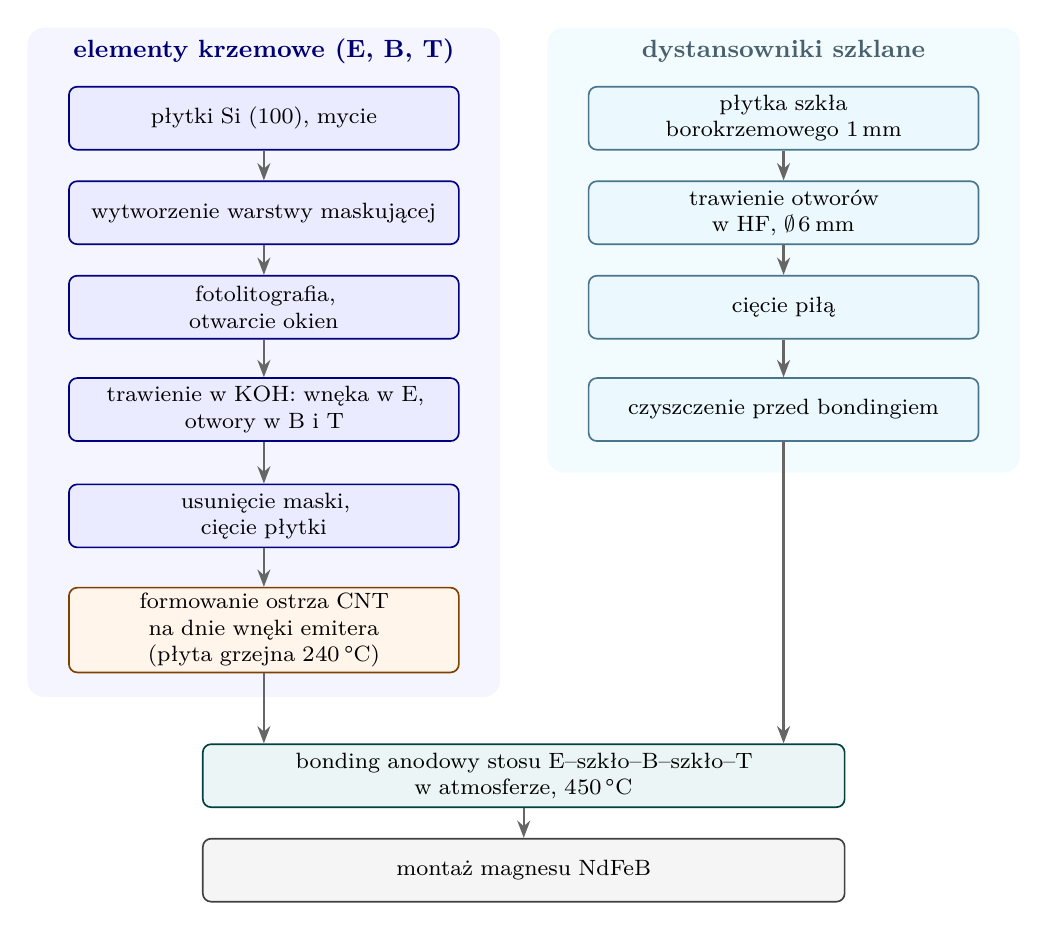
\begin{tikzpicture}[font=\small, >={Stealth[length=2.2mm]},
      krok/.style={draw=#1!50!black, fill=#1!8, rounded corners=3pt, line width=0.6pt,
                   align=center, text width=46mm, minimum height=8mm, inner xsep=5pt, inner ysep=2pt, font=\footnotesize,
                   execute at begin node={\hyphenpenalty=10000\exhyphenpenalty=10000}},
      nr/.style={circle, fill=#1!55!black, text=white, font=\scriptsize\bfseries,
                 inner sep=0pt, minimum size=4.4mm},
      strz/.style={->, line width=0.8pt, draw=black!60}]
    % tła torów
    \fill[blue!4, rounded corners=6pt] (-3.0,0.75) rectangle (3.0,-7.75);
    \fill[cyan!5, rounded corners=6pt] (3.6,0.75) rectangle (9.6,-4.9);
    \node[font=\small\bfseries, text=blue!45!black] at (0,0.45) {elementy krzemowe (E, B, T)};
    \node[font=\small\bfseries, text=cyan!35!black] at (6.6,0.45) {dystansowniki szklane};
    % tor krzemowy
    \node[krok=blue] (s1) at (0,-0.4) {płytki Si (100), mycie};
    \node[krok=blue] (s2) at (0,-1.6) {wytworzenie warstwy maskującej};
    \node[krok=blue] (s3) at (0,-2.8) {fotolitografia,\\otwarcie okien};
    \node[krok=blue] (s4) at (0,-4.1) {trawienie w~KOH: wnęka w~E,\\otwory w~B i~T};
    \node[krok=blue] (s5) at (0,-5.45) {usunięcie maski,\\cięcie płytki};
    \node[krok=orange] (s6) at (0,-6.9) {formowanie ostrza CNT\\na dnie wnęki emitera\\(płyta grzejna \SI{240}{\celsius})};
    % tor szklany
    \node[krok=cyan] (g1) at (6.6,-0.4) {płytka szkła\\borokrzemowego \SI{1}{\milli\metre}};
    \node[krok=cyan] (g2) at (6.6,-1.6) {trawienie otworów\\w~HF, $\varnothing\,\SI{6}{\milli\metre}$};
    \node[krok=cyan] (g3) at (6.6,-2.8) {cięcie piłą};
    \node[krok=cyan] (g4) at (6.6,-4.1) {czyszczenie przed bondingiem};
    % łączenie
    \node[krok=teal, text width=78mm] (b) at (3.3,-8.75)
      {bonding anodowy stosu E--szkło--B--szkło--T\\w~atmosferze, \SI{450}{\celsius}};
    \node[krok=gray, text width=78mm] (m) at (3.3,-9.95) {montaż magnesu NdFeB};
    % strzałki
    \foreach \a/\b in {s1/s2,s2/s3,s3/s4,s4/s5,s5/s6,g1/g2,g2/g3,g3/g4,b/m}
      \draw[strz] (\a) -- (\b);
    \draw[strz] (s6.south) -- (s6.south |- b.north);
    \draw[strz] (g4.south) -- (g4.south |- b.north);
  \end{tikzpicture}
  \caption{Schemat blokowy wytwarzania struktury prototypu \opracowanieWlasne}
  \label{fig:proces}
\end{figure}

\label{sec:szklo}%
Równolegle z~elementami krzemowymi wykonano dystansowniki szklane z~płytki szkła borokrzemowego o~grubości
\SI{1}{\milli\metre}. Najpierw wytrawiono w~niej w~kwasie fluorowodorowym (HF) otwory
o~średnicy \SI{6}{\milli\metre}, przez które przechodzi wiązka elektronów
(\rysref{fig:szklo-otwory}).
Maską była folia ochronna naklejona na szkło, która chroniła pozostałą
powierzchnię przed działaniem HF. Następnie płytkę pocięto piłą na pojedyncze elementy. Taka kolejność
pozwala obrabiać całą płytkę naraz i~zachować jednakowe położenie
otworów we wszystkich dystansownikach. Przed bondingiem elementy
oczyszczono, ponieważ zanieczyszczenia i~nierówności powierzchni
uniemożliwiają szczelne połączenie (\pref{subsec:bonding}).
\TODO{T15: sposób czyszczenia przed bondingiem}

\rysunek[0.75\linewidth]{projekt-prototypu/figures/szklo_otwory_HF.jpg}{Płytka
  szkła borokrzemowego z~dwoma rzędami otworów
  $\varnothing\,\SI{6}{\milli\metre}$ wytrawionych w~HF, przed cięciem
  na dystansowniki; na powierzchni widoczna folia ochronna pełniąca rolę
  maski \opracowanieWlasne}{fig:szklo-otwory}

\label{sec:nanoszenie-cnt}%
Ostatnim etapem przed łączeniem elementów było uformowanie emitera.
Ma on postać ostrza (wieży) z~nanorurek węglowych na dnie wnęki
w~elemencie krzemowym. Zastosowano wodną dyspersję jednościennych
nanorurek węglowych TUBALL BATT H2O firmy OCSiAl Europe S.à~r.l.
(Luksemburg), zawierającą \SI{0.4}{\percent} nanorurek TUBALL,
\SI{0.8}{\percent} dyspersanta PVP i~\SI{98.8}{\percent} wody.
Dyspersant zapobiega aglomeracji nanorurek w~zawiesinie, a~po
odparowaniu wody tworzy z~nimi kompozyt CNT-PVP (\pref{subsec:cnt}).
Zawiesinę nanorurek nakraplano pipetą na element
pomocniczy, który przykładano do emitera nagrzanego na płycie grzejnej
do \SI{240}{\celsius}. Element pomocniczy odciągano następnie szybkim
ruchem od powierzchni emitera. Zawiesina rozciągała się między oboma
elementami i~zasychała w~kontakcie z~gorącym podłożem, tworząc wieżę
nanorurek wydłużoną w~kierunku przyszłej bramki. Wysokość wieży
wynosiła ok.~1,5 grubości dna wnęki emitera, tj.~ok.~\SI{360}{\micro\metre}. Kształt ostrza
zwiększa lokalne natężenie pola na jego wierzchołku (\pref{sec:materialy}).
\TODO{T16: materiał elementu pomocniczego, średnica wieży}

\section{Bonding anodowy i~montaż prototypu}
\label{sec:bonding-montaz}

Elementy połączono bondingiem anodowym w~atmosferze. Płytę grzejną
nagrzewano do \SI{450}{\celsius}, czyli do górnej granicy typowego
zakresu temperatur procesu (\pref{subsec:bonding}). Płyta była
jednocześnie uziemioną elektrodą, a~kolejne warstwy stosu znajdowały
się coraz dalej od niej, więc ich temperatura była niższa niż
temperatura płyty. Wysoka temperatura płyty zapewniała, że także
najwyżej położone połączenia osiągały temperaturę wystarczającą do
przewodnictwa jonowego szkła. Między elementy wprowadzono dodatkowo
przekładkę, która zmniejszała dystans między łączonymi elementami.
\TODO{T18: kolejność łączenia warstw, sposób justowania otworów względem ostrza; czym była przekładka i~gdzie leżała}
\TODO{T19: napięcie i~czas bondingu, czy wszystkie połączenia były trwałe}

Po bondingu pod emiterem zamocowano magnes NdFeB (\rysref{fig:proces}).
\TODO{T20: sposób mocowania magnesu, wymiary i~masa prototypu}

Wszystkie połączenia wykonano w~atmosferze, dlatego wnętrze struktury
nie jest zamknięte w~próżni, a~prototyp jest niehermetyczny. Badania
prowadzono w~komorze próżniowej przy ciśnieniu do
\SI{1e-5}{\milli\bar} (\rozdzref{ch:stanowisko}). Rozwiązaniem
docelowym jest wykonanie ostatniego połączenia bondingiem anodowym
w~próżni i~podtrzymywanie próżni mikropompą; trudności tego procesu
omówiono w~\pref{subsec:bonding}.

Zmontowany prototyp wymaga do pracy zewnętrznej próżni i~zasilania
wysokim napięciem. Stanowisko, na którym go badano, oraz metody
opracowania wyników opisano w~\rozdzref{ch:stanowisko}.

         % 10. prace własne
% Rozdział 4 — Stanowisko pomiarowe i metodyka (budżet: 3,5 str.)
% 17.11.2026 (przegląd spójności): treść zebrana z miejsc, w których była już
% w pracy — p. 2.4.1–2.4.2 i 2.5.5 podstaw teoretycznych (stanowisko,
% charakterystyka I-V, bezpieczeństwo), p. 5.1.4 (metoda analizy zdjęć)
% i p. 5.2.1 (spektrometr). Schemat circuitikz: uklad-pomiarowy/uklad_pomiarowy_body.tex
% (wstawiany makrem \inputBezPreambuly).
\chapter{Stanowisko pomiarowe i~metodyka}
\label{ch:stanowisko}

W~rozdziale opisano stanowisko, na którym badano prototyp, sposób
pomiaru prądów i~napięć oraz metody opracowania zdjęć ekranu
luminescencyjnego i~widm promieniowania X.

\section{Komora próżniowa i~obwód elektryczny}
\label{sec:obwod}

\begin{zmiana}
Struktura prototypu jest otwarta, tak jak w~docelowym przyrządzie
pracującym w~próżni kosmicznej, dlatego wszystkie pomiary prowadzono
w~komorze próżniowej. Ciśnienie
w~komorze podczas pomiarów nie przekraczało \SI{1e-5}{\milli\bar}
(\SI{1e-3}{\pascal}), co zapewnia propagację wiązki bez zderzeń
z~cząsteczkami gazu (\pref{sec:emisja}).
\end{zmiana}
\usun{„Prototyp nie jest hermetyczny” (U33)}

\begin{przeniesione}
W~badanym układzie emisję wywołuje napięcie ekstrakcyjne $\UB$
przyłożone między emiter (E) a~bramkę (B) z~otworem. Poniżej napięcia
progowego prąd emisji jest niemierzalny, a~powyżej progu rośnie
wykładniczo zgodnie z~\eqref{eq:fn}. Część elektronów trafia w~bramkę,
a~część przechodzi przez otwór i~jest przyspieszana w~stronę targetu (T)
napięciem przyspieszającym $\UT$, które decyduje o~energii elektronów
padających na próbkę.
\end{przeniesione}
\przen{U15, U17: z~dawnych p.~2.2.4 i~2.3.2}

Schemat obwodu elektrycznego przedstawiono na \rysref{fig:uklad-pomiarowy}.
Emiter (E) jest wspólnym punktem obu obwodów i~znajduje się na
potencjale masy. Zasilacz~1 doprowadza do targetu (T) dodatnie napięcie
przyspieszające $\UT$, a~zasilacz~2 do bramki (B) dodatnie napięcie
ekstrakcyjne $\UB$.
\begin{przeniesione}
Target musi mieć potencjał dodatni względem emitera, co można uzyskać
także, uziemiając target i~polaryzując emiter napięciem $-\UT$. Ten
wariant jest prostszy w~realizacji: próbka, uchwyt i~komora pozostają
na potencjale masy, więc między próbką a~detektorem nie występuje pole
odchylające elektrony ani ryzyko przebicia do detektora. Wymaga on
jednak zasilacza wysokiego napięcia o~ujemnej polaryzacji wyjścia,
a~obwód bramki musi być wtedy odniesiony do potencjału emitera.
\end{przeniesione}
\przen{U17: warianty polaryzacji z~dawnego p.~2.3.2}

\begin{figure}[htbp]
  \centering
  \resizebox{\textwidth}{!}{\inputBezPreambuly{../uklad-pomiarowy/uklad_pomiarowy_body}}
  \caption{Schemat układu do pomiaru emisji polowej w~prototypie analizatora EDS:
    E -- emiter, B -- bramka (elektroda ekstrakcyjna), T -- target;
    $\UT$ -- zasilacz obwodu targetu, $\UB$ -- zasilacz bramki;
    $\RT$, $\RB$ -- rezystory ograniczające, V -- woltomierze
}
  \label{fig:uklad-pomiarowy}
\end{figure}

W~każdym obwodzie znajduje się rezystor ograniczający
$\RT = \RB = \SI{100}{\kilo\ohm}$. Rezystory ograniczają prąd w~razie
wyładowania między elektrodami, a~jednocześnie służą do pomiaru prądu:
woltomierz mierzy spadek napięcia na rezystorze, a~prąd oblicza się
z~prawa Ohma (\SI{1}{\volt} na rezystorze odpowiada
\SI{10}{\micro\ampere}). Prąd emisji $\Ie$ podawany w~\rozdzref{ch:badania}
jest prądem w~obwodzie targetu, obliczonym z~napięcia na $\RT$.
Niepewność pomiaru prądu wynika z~klasy woltomierza i~tolerancji
rezystora, a~niepewność napięć z~dokładności nastaw zasilaczy.

Charakterystyki emisji mierzono przy stałym napięciu $\UT$
(\SI{2000}{\volt} w~sesji bez magnesu, \SI{1500}{\volt}
i~\SI{10}{\kilo\volt} w~sesjach z~magnesem), zwiększając $\UB$ co \SI{100}{\volt} w~zakresie
\SIrange{500}{1700}{\volt}. Z~charakterystyki $\Ie(\UB)$ odczytuje się
napięcie progowe emisji i~największy prąd. Widma rejestrowano przy
$\UT = \SI{4}{\kilo\volt}$ ($\UB = \SI{1}{\kilo\volt}$) oraz
$\UT = \SI{10}{\kilo\volt}$.

\section{Obserwacja wiązki i~analiza zdjęć ekranu}
\label{sec:analiza-zdjec}

\begin{przeniesione}
Kształt i~położenie wiązki obserwuje się na ekranie pokrytym luminoforem,
który świeci w~miejscu padania elektronów. Jasność świecenia rośnie
z~gęstością prądu, dlatego zdjęcie ekranu pokazuje rozkład gęstości
prądu w~przekroju wiązki. Metoda ta jest jakościowa: jasność zależy też
od energii elektronów, rodzaju luminoforu, jego degradacji i~ustawień
aparatu.
\end{przeniesione}
\przen{U18: z~dawnego p.~2.3.6}

Kształt wiązki obserwowano na ekranie luminescencyjnym, czyli warstwie
luminoforu umieszczonej w~miejscu próbki. Ekran
fotografowano kamerą z~automatyczną ekspozycją przy kolejnych
napięciach $\UB$ z~serii pomiarowej.

Luminescencja ekranu ma barwę niebieską, a~tło (podświetlenie,
żarnik) -- pomarańczowo-czerwoną. Dla każdego piksela obliczono
nadmiar składowej niebieskiej
\begin{equation}
  \Delta = \max\bigl(0,\; C_\mathrm{n} - \max(C_\mathrm{c}, C_\mathrm{z})\bigr),
  \label{eq:nadmiar-niebieskiego}
\end{equation}
gdzie $C_\mathrm{c}$, $C_\mathrm{z}$, $C_\mathrm{n}$ to składowe
czerwona, zielona i~niebieska koloru (0--255). Za obszar plamki uznano
piksele z~$\Delta > 40$. Na tej podstawie obliczono dwie wielkości:
\begin{itemize}
  \item jasność świecenia $L = \frac{1}{N}\sum \Delta$, czyli sumę nadmiaru
        niebieskiego podzieloną przez liczbę pikseli kadru $N$ (w~jednostkach
        umownych, j.u.),
  \item pole plamki, czyli udział pikseli plamki w~kadrze [\%].
\end{itemize}

Związek jasności z~prądem oceniano współczynnikiem korelacji Pearsona
$r_\mathrm{P}$. Ze względu na automatyczną ekspozycję i~różne
kadrowanie w~poszczególnych sesjach wartości bezwzględne nie są wprost
porównywalne między sesjami; porównuje się trendy i~wielkości względne.

\section{Rejestracja widm promieniowania X}
\label{sec:rejestracja-widm}

Do rejestracji widm użyto spektrometru rentgenowskiego KETEK AXAS-D
(KETEK GmbH, Monachium) z~detektorem SDD, skierowanego na obszar próbki, na który pada
wiązka. Impulsy z~detektora przetwarzał cyfrowy procesor impulsów
KETEK DPP2 obsługiwany programem ProSpect, który zapisuje widmo jako
liczbę zliczeń w~\num{8192} kanałach. Ustawienia akwizycji podano
w~\pref{sec:widma-warunki}. Skalę energii korygowano liniowo na
podstawie położeń linii o~jednoznacznej identyfikacji, a~widma
analizowano jakościowo, przypisując piki pierwiastkom
(\pref{sec:spektrometria}).

\usun{p.~„Bezpieczeństwo pracy” (U32)}

\ifdefined\wersjaPrezentacja
  % Rozdział 5 — WERSJA „PREZENTACJA” (main-prezentacja.tex), 22.11.2026 (kris):
% same wyniki z parametrami pomiarów, bez interpretacji, z pustym
% podrozdziałem „Wnioski”. Pełna wersja: rozdzialy/05_badania.tex.
% Dane i rysunki te same co w emisja_tresc.tex, widma_tresc.tex
% i widma_materialy_tresc.tex — przy zmianach danych poprawić oba pliki.
\chapter{Badania eksperymentalne}
\label{ch:badania}

\renewcommand{\figdir}{../emisja-magnes-pomiary/figures}
\renewcommand{\datadir}{../emisja-magnes-pomiary/dane}
\providecommand{\sesjaM}{z~magnesem}
\providecommand{\sesjaB}{bez magnesu}
\pgfplotsset{/pgf/number format/use comma, /pgf/number format/1000 sep={}}

W~rozdziale przedstawiono wyniki pomiarów emisji polowej prototypu
z~magnesem ogniskującym i~bez niego oraz widma promieniowania X
zarejestrowane dla próbek o~różnym składzie. Stanowisko i~metody opisano
w~\rozdzref{ch:stanowisko}.

\section{Wpływ magnesu ogniskującego na emisję polową}
\label{sec:emisja-magnes}

\subsection{Przebieg pomiarów}

Wykonano sesje pomiarowe, w~których przy stałym napięciu $\UT$
zwiększano napięcie $\UB$ co \SI{100}{V} i~rejestrowano prąd emisji
$\Ie$ oraz zdjęcie ekranu luminescencyjnego (\rozdzref{ch:stanowisko}):
\begin{itemize}
  \item \textbf{sesja bez magnesu} -- $\UT=\SI{2000}{V}$,
        $\UB$ od \SI{500}{V} do \SI{1500}{V}, zdjęcia dla $\UB$ od
        \SI{700}{V} do \SI{1100}{V}; przed sesją źródło odgazowano
        przez wygrzanie w~temperaturze ok. \SI{200}{\celsius},
  \item \textbf{sesja z~magnesem} -- $\UT=\SI{1500}{V}$,
        $\UB$ od \SI{500}{V} do \SI{1700}{V}, zdjęcia dla $\UB$ od
        \SI{500}{V} do \SI{1600}{V}; bez ponownego odgazowania źródła,
  \item \textbf{seria z~magnesem przy $\UT=\SI{10}{kV}$} --
        $\UB$ od \SI{600}{V} do \SI{1400}{V}, bez zdjęć ekranu.
\end{itemize}

Dodatkowo wykonano serię~2 bez magnesu z~odczytami prądu od
\SI{1}{\micro A} do \SI{400}{\micro A}. Ciśnienie w~komorze nie
przekraczało \SI{1e-5}{\milli\bar}. Zmierzone prądy zestawiono
w~tab.~\ref{tab:emisja-iv}.

\begin{table}[htbp]
  \centering
  \caption{Prąd emisji w~funkcji napięcia $\UB$ w~sesjach pomiarowych}
  \label{tab:emisja-iv}
  \begin{tabular}{@{}r r r r@{}}
    \toprule
    $\UB$ [V] & $\Ie$ \sesjaB\ [µA] & $\Ie$ \sesjaM\ [µA] & $\Ie$ \sesjaM\ [µA] \\
    \midrule
     500 & 0    & 14 & -- \\
     600 & 0    & 16 & 4 \\
     700 & 0    & 14 & 18 \\
     800 & 2    & 28 & 36 \\
     900 & 3,1  & 45 & 44 \\
    1\,000 & 4    & 69 & 99 \\
    1\,100 & 6    & 118 & 127 \\
    1\,200 & 8    & 180 & 127 \\
    1\,300 & 9    & 190 & 126 \\
    1\,400 & 11,2 & 190 & 125 \\
    1\,500 & 22   & 193 & -- \\
    1\,600 & --   & 200 & -- \\
    1\,700 & --   & 200 & -- \\
    \midrule
    $\UT$ & \SI{2000}{V} & \SI{1500}{V} & \SI{10}{kV} \\
    \bottomrule
  \end{tabular}
\end{table}

\subsection{Charakterystyki prądowo-napięciowe}

Charakterystyki $\Ie(\UB)$ wszystkich sesji przedstawiono na rys.~\ref{fig:emisja-iv}.

\begin{figure}[htbp]
  \centering
  \begin{tikzpicture}
    \begin{semilogyaxis}[
      width=0.85\textwidth, height=7cm,
      xlabel={napięcie $\UB$ [V]}, ylabel={prąd emisji $\Ie$ [µA]},
      xmin=450, xmax=1750, ymin=1, ymax=500, xtick distance=200,
      grid=major, grid style={gray!25},
      legend pos=south east, legend cell align=left,
      every axis plot/.append style={thick, mark size=2pt},
      unbounded coords=jump,
    ]
      \addplot[red!60!black, mark=triangle*] table[x=U,y=I_uA,col sep=comma]{\datadir/iv_bez.csv};
      \addlegendentry{\sesjaB\ ($\UT=\SI{2000}{V}$)}
      \addplot[blue!70!black, mark=*] table[x=U,y=I_uA,col sep=comma]{\datadir/iv_mag.csv};
      \addlegendentry{\sesjaM\ ($\UT=\SI{1500}{V}$)}
      \addplot[black, mark=diamond*, mark size=2.6pt] table[x=U,y=I_uA,col sep=comma]{\datadir/iv_10kV.csv};
      \addlegendentry{\sesjaM\ ($\UT=\SI{10}{kV}$)}
    \end{semilogyaxis}
  \end{tikzpicture}
  \caption{Prąd emisji w~funkcji napięcia $\UB$: \sesjaB\ przy
    $\UT=\SI{2000}{V}$, \sesjaM\ przy $\UT=\SI{1500}{V}$
    i~$\UT=\SI{10}{kV}$
    (skala logarytmiczna; punkty z~$\Ie=0$ pominięto)}
  \label{fig:emisja-iv}
\end{figure}

\section{Obserwacja wiązki na ekranie luminescencyjnym}
\label{sec:emisja-ekran}

Wpływ magnesu na kształt wiązki oceniono na podstawie zdjęć ekranu
luminescencyjnego wykonanych w~sesjach opisanych w~\pref{sec:emisja-magnes}.

\subsection{Jasność ekranu}

Jasność świecenia ekranu $L$ wyznaczono ze zdjęć metodą opisaną
w~\pref{sec:analiza-zdjec}. Jej zależność od napięcia $\UB$ w~obu
sesjach przedstawiono na rys.~\ref{fig:emisja-I}, a~zależność od
odczytu prądu w~serii~2 na rys.~\ref{fig:emisja-IvsIe}.

\begin{figure}[htbp]
  \centering
  \begin{tikzpicture}
    \begin{axis}[
      width=0.8\textwidth, height=6.5cm,
      xlabel={napięcie $\UB$ [V]}, ylabel={jasność $L$ [j.u.]},
      xmin=450, xmax=1650, ymin=0, ymax=3.5, xtick distance=200,
      grid=major, grid style={gray!25},
      legend pos=north west, legend cell align=left,
      every axis plot/.append style={thick, mark size=2pt},
    ]
      \addplot[blue!70!black, mark=*] table[x=U,y=I,col sep=comma]{\datadir/mg.csv};
      \addlegendentry{\sesjaM\ ($\UT=\SI{1500}{V}$)}
      \addplot[red!60!black, mark=triangle*] table[x=U,y=I,col sep=comma]{\datadir/s1.csv};
      \addlegendentry{\sesjaB\ ($\UT=\SI{2000}{V}$)}
    \end{axis}
  \end{tikzpicture}
  \caption{Jasność świecenia ekranu w~funkcji napięcia $\UB$:
    \sesjaM\ przy $\UT=\SI{1500}{V}$, \sesjaB\ przy $\UT=\SI{2000}{V}$}
  \label{fig:emisja-I}
\end{figure}

\begin{figure}[htbp]
  \centering
  \begin{tikzpicture}
    \begin{loglogaxis}[
      width=0.65\textwidth, height=5.5cm,
      xtick={30,50,100,200,400}, xticklabels={30,50,100,200,400},
      log ticks with fixed point,
      xlabel={prąd emisji $\Ie$ [µA]},
      ylabel={jasność $L$ [j.u.]},
      grid=major, grid style={gray!25},
    ]
      \addplot[only marks, mark=square*, orange!85!black]
        table[x=etykieta, y=I, col sep=comma,
              restrict expr to domain={\thisrow{I}}{0.01:100}]{\datadir/s2.csv};
    \end{loglogaxis}
  \end{tikzpicture}
  \caption{Jasność świecenia ekranu w~funkcji odczytu prądu emisji,
    seria~2 \sesjaM}
  \label{fig:emisja-IvsIe}
\end{figure}

\subsection{Obraz plamki}

Zdjęcia ekranu z~obu sesji przy napięciach $\UB$ od \SI{800}{V} do
\SI{1100}{V} zestawiono na rys.~\ref{fig:emisja-sbs}, zdjęcia z~sesji
z~magnesem przy \SI{700}{V}, \SI{1400}{V} i~\SI{1600}{V} na
rys.~\ref{fig:emisja-mg-skrajne}, a~pełne kadry na
rys.~\ref{fig:emisja-pelne}. Parametry emisji i~plamki podano
w~tab.~\ref{tab:emisja}.

\begin{table}[htbp]
  \centering
  \caption{Parametry emisji i~plamki w~obu sesjach}
  \label{tab:emisja}
  \begin{tabular}{@{}lccc@{}}
    \toprule
    Parametr & \sesjaM & \sesjaB & seria 2 (\sesjaM) \\
    \midrule
    Odgazowanie źródła & nie & tak (\SI{200}{\celsius}) & tak (\SI{200}{\celsius}) \\
    Napięcie $\UT$ & \SI{1500}{V} & \SI{2000}{V} & \SI{2000}{V} \\
    Pierwsza widoczna plamka & \SI{600}{V} & \SI{800}{V} & \SI{700}{V} \\
    Prąd maksymalny & \SI{200}{\micro A} & \SI{22}{\micro A} & \SI{400}{\micro A} \\
    Maks. jasność $L$ [j.u.] & 3,19 & 1,67 & 2,89 \\
    Maks. pole plamki [\% kadru] & 3,98 & 2,07 & 3,91 \\
    \bottomrule
  \end{tabular}
\end{table}

\newcommand{\sbs}[2]{%
  \begin{subfigure}[t]{0.28\textwidth}\centering
    \includegraphics[width=\linewidth]{\figdir/#1}\caption{#2}
  \end{subfigure}}

\begin{figure}[p]
  \centering
  \makebox[0.28\textwidth]{\textbf{\sesjaM}}\hspace{1.5em}\makebox[0.28\textwidth]{\textbf{\sesjaB}}\par\medskip
  \sbs{mg_03.jpg}{\SI{800}{V}, \SI{28}{\micro A}}\hspace{1.5em}
  \sbs{s1_02.jpg}{\SI{800}{V}, \SI{2}{\micro A}}\par\medskip
  \sbs{mg_04.jpg}{\SI{900}{V}, \SI{45}{\micro A}}\hspace{1.5em}
  \sbs{s1_03.jpg}{\SI{900}{V}, \SI{3,1}{\micro A}}\par\medskip
  \sbs{mg_05.jpg}{\SI{1000}{V}, \SI{69}{\micro A}}\hspace{1.5em}
  \sbs{s1_04.jpg}{\SI{1000}{V}, \SI{4}{\micro A}}\par\medskip
  \sbs{mg_06.jpg}{\SI{1100}{V}, \SI{118}{\micro A}}\hspace{1.5em}
  \sbs{s1_05.jpg}{\SI{1100}{V}, \SI{6}{\micro A}}
  \caption{Zbliżenia okna ekranu \sesjaM\ ($\UT=\SI{1500}{V}$, lewa kolumna)
    i~\sesjaB\ ($\UT=\SI{2000}{V}$, prawa kolumna) przy tych samych
    napięciach $\UB$; podpisy: $\UB$, $\Ie$}
  \label{fig:emisja-sbs}
\end{figure}

\begin{figure}[htbp]
  \centering
  \begin{subfigure}[t]{0.28\textwidth}\centering
    \includegraphics[width=\linewidth]{\figdir/mg_02.jpg}\caption{\SI{700}{V}}\end{subfigure}\hspace{1.5em}
  \begin{subfigure}[t]{0.28\textwidth}\centering
    \includegraphics[width=\linewidth]{\figdir/mg_09.jpg}\caption{\SI{1400}{V}}\end{subfigure}\hspace{1.5em}
  \begin{subfigure}[t]{0.28\textwidth}\centering
    \includegraphics[width=\linewidth]{\figdir/mg_11.jpg}\caption{\SI{1600}{V}}\end{subfigure}
  \caption{Ekran w~sesji \sesjaM\ ($\UT=\SI{1500}{V}$) przy
    $\UB = \SI{700}{V}$, \SI{1400}{V} i~\SI{1600}{V}}
  \label{fig:emisja-mg-skrajne}
\end{figure}

\begin{figure}[htbp]
  \centering
  \begin{subfigure}[t]{0.32\textwidth}\centering
    \includegraphics[width=\linewidth]{\figdir/mg_pelny.jpg}\caption{\sesjaM, \SI{1400}{V}}\end{subfigure}\hfill
  \begin{subfigure}[t]{0.32\textwidth}\centering
    \includegraphics[width=\linewidth]{\figdir/s1_pelny.jpg}\caption{\sesjaB, \SI{1100}{V}}\end{subfigure}\hfill
  \begin{subfigure}[t]{0.32\textwidth}\centering
    \includegraphics[width=\linewidth]{\figdir/s2_pelny.jpg}\caption{\sesjaM, seria 2}\end{subfigure}
  \caption{Pełne kadry ekranu przy największym prądzie w~każdej serii}
  \label{fig:emisja-pelne}
\end{figure}

\subsection{Wnioski}

\vspace{6\baselineskip}

\section{Widma EDS próbek}
\label{sec:widma}

\subsection{Widmo próbki aluminiowej przy $\UT = \SI{4}{\kilo\volt}$}
\label{sec:widma-warunki}\label{sec:widma-linie}\label{sec:widma-stabilnosc}

Widmo zarejestrowano 12.06.2026 dla płytki aluminiowej, z~magnesem
ogniskującym na emiterze, przy prądzie emisji $\Ie \approx
\SI{100}{\micro\ampere}$ i~ciśnieniu nie większym niż
\SI{1e-5}{\milli\bar}, spektrometrem opisanym
w~\pref{sec:rejestracja-widm}. Parametry pomiaru zestawiono
w~\tabref{tab:widma-parametry}, widmo przedstawiono na
\rysref{fig:widmo-4kV}, zidentyfikowane linie w~\tabref{tab:widma-linie},
a~przebieg częstości zliczeń w~czasie pomiaru na \rysref{fig:widma-stabilnosc}.

\begin{table}[htbp]\centering
  \caption{Parametry rejestracji widma EDS}\label{tab:widma-parametry}
  \begin{tabular}{@{}ll@{}}\toprule
    Parametr & Wartość \\\midrule
    Napięcie przyspieszające $\UT$ & \SI{4000}{\volt} \\
    Napięcie ekstrakcyjne $\UB$ & \SI{1000}{\volt} \\
    Prąd emisji $\Ie$ & ok.~\SI{100}{\micro\ampere} \\
    Czas kształtowania (\angielski{peaking time}) & \SI{0.5}{\micro\second} \\
    Liczba kanałów, szerokość kanału & \num{8192}, \SI{10}{\electronvolt} \\
    Czas rzeczywisty / czas życia & \SI{210.7}{\second} / \SI{100.1}{\second} \\
    Częstość zliczeń wejściowa / wyjściowa & ok.~475~kcps / ok.~225~kcps \\
    Czas martwy & \SIrange{52}{54}{\percent} \\\bottomrule
  \end{tabular}
\end{table}

\rysunek[0.95\linewidth]{widma-eds/widmo_eds_4kV.pdf}{Widmo EDS płytki
  aluminiowej przy $\UT=\SI{4}{\kilo\volt}$ i~$\UB=\SI{1}{\kilo\volt}$,
  czas życia \SI{100}{\second}}{fig:widmo-4kV}

\begin{table}[htbp]\centering
  \caption{Linie zidentyfikowane w~widmie z~\rysref{fig:widmo-4kV}}\label{tab:widma-linie}
  \begin{tabular}{@{}S[table-format=1.2]lS[table-format=1.3]@{}}\toprule
    {$E$ piku [\si{\kilo\electronvolt}]} & Linia & {$E$ tabel. [\si{\kilo\electronvolt}]} \\\midrule
    1.26 & Mg~\Ka & 1.254 \\
    1.48 & Al~\Ka & 1.487 \\
    1.74 & Si~\Ka & 1.740 \\
    2.98 & Al~\Ka{} + Al~\Ka & 2.974 \\
    3.22 & Al~\Ka{} + Si~\Ka & 3.227 \\
    3.46 & Si~\Ka{} + Si~\Ka & 3.480 \\\bottomrule
  \end{tabular}
\end{table}

\rysunek[0.9\linewidth]{widma-eds/stabilnosc_zliczen.pdf}{Częstość zliczeń
  wejściowa (ICR), wyjściowa (OCR) i~średnia częstość w~kanale Al~\Ka{}
  w~czasie rejestracji widma przy $\UT=\SI{4}{\kilo\volt}$
}{fig:widma-stabilnosc}

\subsection{Widma próbek o~różnym składzie przy $\UT = \SI{10}{\kilo\volt}$}
\label{sec:widma-probki}\label{sec:widma-tlen}

Widma zarejestrowano 13.11.2026 przy $\UT=\SI{10}{\kilo\volt}$ dla
czterech próbek: A~(miedź o~nieznanym składzie), B~(ołów), C~(złoto,
chrom i~miedź) i~D~(aluminium). Dla próbek A--C wykonano po 6--10 serii
o~czasie życia \SIrange{40}{250}{\second}, które zsumowano; dla
próbki~D wykorzystano serię o~czasie martwym \SI{20}{\percent}. Skalę
energii skorygowano liniowo na podstawie położeń linii Al~\Ka,
Pb~M$\alpha$, Cr~\Ka, Fe~\Ka{} i~Cu~\Ka. Widma przedstawiono na
\rysref{fig:widma-probki}, a~zidentyfikowane linie w~\tabref{tab:widma-probki}.

\rysunek[0.95\linewidth]{widma-eds/widma_materialy.pdf}{Widma EDS próbek A, B i~C
  przy $\UT=\SI{10}{\kilo\volt}$ (13.11.2026, skala logarytmiczna, zliczenia
  na sekundę czasu życia)}{fig:widma-probki}

\begin{table}[htbp]\centering\small
  \caption{Linie zidentyfikowane w~widmach z~13.11.2026}\label{tab:widma-probki}
  \begin{tabular}{@{}lll@{}}\toprule
    Próbka & Pierwiastek & Linie i~energie po korekcji [\si{\kilo\electronvolt}] \\\midrule
    A & Cu       & L$\alpha$ 0,92; \Ka{} 8,04; \Kb{} 8,90 \\
      & Te       & L$\alpha$ 3,76; L$\beta_1$ 4,04; L$\beta_2$ 4,30; L$\gamma_1$ 4,57 \\
      & P        & \Ka{} 2,01 \\
      & S, Cl, K & \Ka{} 2,30; 2,62; 3,32 \\
      & Si, Al   & \Ka{} 1,73; 1,48 \\\midrule
    B & Pb       & M$\zeta$ 1,83; M$\alpha$ 2,35; M$\gamma$ 2,65 \\\midrule
    C & Au       & M$\zeta$ 1,66; M$\alpha\beta$ 2,13; M$\gamma$ 2,41 \\
      & Cr       & \Ka{} 5,42; \Kb{} 5,95 \\
      & Cu       & L$\alpha$ 0,93; \Ka{} 8,04 \\\midrule
    D & Al       & \Ka{} 1,48 \\
      & Mn, Fe   & \Ka{} 5,91; 6,40 \\
      & --       & pik sumacyjny 2,98 \\\bottomrule
  \end{tabular}
\end{table}
 % rozdz. 5 bez interpretacji (main-prezentacja.tex)
\else
  % Rozdział 5 — Badania eksperymentalne (budżet: 13 str.)
% 5.1 Źródło: emisja-magnes-pomiary/emisja_tresc.tex (zaczyna się od \section).
% Fragment używa \figdir i \datadir — ustawiane tutaj względem wspolne/.
\chapter{Badania eksperymentalne}
\label{ch:badania}

W~rozdziale przedstawiono wyniki pomiarów emisji polowej prototypu
z~magnesem ogniskującym i~bez niego oraz widma promieniowania X
wzbudzanego wiązką elektronów w~próbkach o~różnym składzie. Stanowisko
i~metody opisano w~\rozdzref{ch:stanowisko}.

\renewcommand{\figdir}{../emisja-magnes-pomiary/figures}
\renewcommand{\datadir}{../emisja-magnes-pomiary/dane}
% =====================================================================
%  Emisja polowa: sesja z magnesem vs. sesje bez magnesu
%  17.11.2026: U -> \UB, intensywność I -> jasność L, e -> \Delta, r -> r_P,
%  sesje nazywane „bez magnesu”/„z magnesem” (nie B/M: B = bramka),
%  bez nazw plików roboczych; metoda analizy zdjęć przeniesiona do rozdz. 4.
%  Fragment do wstawienia w rozdział 5 (\input{...}).
%  Wymaga: graphicx, subcaption, pgfplots (compat>=1.17), booktabs, siunitx
%  Ścieżki: figures/ (zdjęcia), dane/ (CSV z pomiarów i analizy obrazu)
% =====================================================================
\providecommand{\sesjaM}{z~magnesem}
\providecommand{\sesjaB}{bez magnesu}
\providecommand{\figdir}{figures}
\providecommand{\datadir}{dane}
\pgfplotsset{/pgf/number format/use comma, /pgf/number format/1000 sep={}}
\providecommand{\TODO}[1]{\textcolor{red}{[TODO: #1]}}

\section{Wpływ magnesu ogniskującego na emisję polową}
\label{sec:emisja-magnes}

\subsection{Przebieg pomiarów i~charakterystyki prądowo-napięciowe}

Porównano dwie sesje pomiarowe, w~których przy stałym napięciu $\UT$
zwiększano napięcie $\UB$ co \SI{100}{V} i~rejestrowano prąd emisji
$\Ie$ oraz zdjęcie ekranu luminescencyjnego (\rozdzref{ch:stanowisko}):
\begin{itemize}
  \item \textbf{sesja bez magnesu} -- $\UT=\SI{2000}{V}$,
        $\UB=\SIrange{500}{1500}{V}$, prąd w~zakresie
        \SIrange{2}{22}{\micro A}, zdjęcia dla
        $\UB=\SIrange{700}{1100}{V}$; przed tą sesją źródło odgazowano
        przez wygrzanie w~temperaturze ok. \SI{200}{\celsius},
  \item \textbf{sesja z~magnesem} -- $\UT=\SI{1500}{V}$,
        $\UB=\SIrange{500}{1700}{V}$, prąd w~zakresie
        \SIrange{14}{200}{\micro A}, zdjęcia dla
        $\UB=\SIrange{500}{1600}{V}$; źródło nie było przed tą sesją
        ponownie odgazowane.
\end{itemize}
Dodatkowo wykorzystano serię~2 bez magnesu (10~zdjęć z~odczytami prądu
\SIrange{1}{400}{\micro A}), która posłużyła do sprawdzenia związku jasności
ekranu z~prądem. Wyniki zebrano w~tab.~\ref{tab:emisja-iv}.

\begin{table}[htbp]
  \centering
  \caption{Prąd emisji w~funkcji napięcia w~obu sesjach}
  \label{tab:emisja-iv}
  \begin{tabular}{@{}r r r@{}}
    \toprule
    $\UB$ [V] & $\Ie$ \sesjaB\ [µA] & $\Ie$ \sesjaM\ [µA] \\
    \midrule
     500 & 0    & 14 \\
     600 & 0    & 16 \\
     700 & 0    & 14 \\
     800 & 2    & 28 \\
     900 & 3,1  & 45 \\
    1000 & 4    & 69 \\
    1100 & 6    & 118 \\
    1200 & 8    & 180 \\
    1300 & 9    & 190 \\
    1400 & 11,2 & 190 \\
    1500 & 22   & 193 \\
    1600 & --   & 200 \\
    1700 & --   & 200 \\
    \midrule
    $\UT$ & \SI{2000}{V} & \SI{1500}{V} \\
    \bottomrule
  \end{tabular}
\end{table}

Uzyskane charakterystyki $\Ie(\UB)$ przedstawiono na rys.~\ref{fig:emisja-iv}.
W~sesji bez magnesu prąd pojawia się skokowo przy \SI{800}{V} i~rośnie niemal
liniowo do \SI{1400}{V}; punkt \SI{1500}{V} (\SI{22}{\micro A}, podwojenie
prądu) odbiega od trendu i~może wskazywać na początek wyładowania
lub niestabilności emisji. W~sesji z~magnesem dla $\UB\leq\SI{700}{V}$ płynie
stały prąd ok. \SI{15}{\micro A}, który należy traktować jako prąd
upływu (tło), następnie prąd rośnie wykładniczo do \SI{180}{\micro A}
przy \SI{1200}{V}, po czym nasyca się na poziomie
\SIrange{190}{200}{\micro A}. Przy tym samym napięciu $\UB$ prąd w~sesji
z~magnesem jest ok. 10--20 razy większy niż bez magnesu (np. \SI{69}{\micro A} wobec
\SI{4}{\micro A} przy \SI{1000}{V}), mimo niższego $\UT$.

Interpretację tych wyników utrudnia to, że sesje nie różnią się wyłącznie obecnością magnesu. Przed sesją bez
magnesu źródło odgazowano, a~przed sesją z~magnesem nie powtórzono tej
procedury. Gazy zaadsorbowane na powierzchni emitera i~elementów
źródła zmieniają pracę wyjścia emitera i~mogą być desorbowane pod
wpływem wiązki, lokalnie zwiększając ciśnienie (\pref{sec:emisja}).
Prawdopodobnie dlatego w~sesji z~magnesem obserwuje się:
\begin{itemize}
  \item stały prąd ok. \SI{15}{\micro A} już przy \SI{500}{V}, przed
        właściwym progiem emisji (upływ lub prąd jonowy),
  \item nasycenie prądu powyżej \SI{1200}{V},
  \item rozległą, rozmytą poświatę wokół plamki, która może być
        częściowo świeceniem gazu resztkowego.
\end{itemize}
Wyższy prąd w~sesji z~magnesem może wynikać z~dwóch przyczyn, których na
podstawie tych pomiarów nie da się rozdzielić: ogniskowania wiązki
przez magnes (więcej elektronów trafia w~target zamiast w~elektrody
i~ścianki źródła) oraz innego stanu powierzchni emitera i~ciśnienia
w~nieodgazowanym źródle, łącznie z~udziałem prądu upływu. Dlatego
wpływ magnesu oceniono przede wszystkim na podstawie kształtu
i~skupienia plamki.

\begin{figure}[htbp]
  \centering
  \begin{tikzpicture}
    \begin{semilogyaxis}[
      width=0.85\textwidth, height=7cm,
      xlabel={napięcie $\UB$ [V]}, ylabel={prąd emisji $\Ie$ [µA]},
      xmin=450, xmax=1750, ymin=1, ymax=500, xtick distance=200,
      grid=major, grid style={gray!25},
      legend pos=south east, legend cell align=left,
      every axis plot/.append style={thick, mark size=2pt},
      unbounded coords=jump,
    ]
      \addplot[red!60!black, mark=triangle*] table[x=U,y=I_uA,col sep=comma]{\datadir/iv_bez.csv};
      \addlegendentry{\sesjaB\ ($\UT=\SI{2000}{V}$)}
      \addplot[blue!70!black, mark=*] table[x=U,y=I_uA,col sep=comma]{\datadir/iv_mag.csv};
      \addlegendentry{\sesjaM\ ($\UT=\SI{1500}{V}$)}
      \draw[gray, dashed] (axis cs:450,15) -- (axis cs:1750,15)
        node[pos=0.2, below, font=\scriptsize] {upływ ok. \SI{15}{\micro A}};
    \end{semilogyaxis}
  \end{tikzpicture}
  \caption{Charakterystyki prądowo-napięciowe emisji w~obu sesjach
    (skala logarytmiczna; punkty z~$\Ie=0$ pominięto)}
  \label{fig:emisja-iv}
\end{figure}


\subsection{Obraz wiązki na ekranie luminescencyjnym}

Jasność świecenia ekranu $L$ wyznaczono ze zdjęć metodą opisaną
w~\pref{sec:analiza-zdjec}. Na rys.~\ref{fig:emisja-I} zestawiono ją
z~prądem emisji w~funkcji napięcia. W~sesji bez magnesu jasność ekranu
rośnie razem z~prądem ($r_\mathrm{P}=0{,}99$ dla \SIrange{800}{1100}{V}).
W~sesji z~magnesem $r_\mathrm{P}=0{,}95$ dla \SIrange{800}{1200}{V}, a~powyżej
\SI{1200}{V} zarówno prąd, jak i~jasność przestają rosnąć -- nasycenie
prądu jest więc rzeczywiste, a~nie wynika tylko z~prześwietlenia
kamery. W~sesji z~magnesem słaba plamka jest widoczna już
przy \SIrange{600}{700}{V}, gdy mierzony prąd nie odbiega jeszcze od
poziomu upływu -- magnes skupia niewielki prąd emisji na małym
obszarze ekranu, przez co staje się on widoczny wcześniej niż bez
magnesu (próg \SI{800}{V}). Dla serii~2 \sesjaB\ korelacja jasności
z~odczytem prądu wynosi $r_\mathrm{P}=0{,}98$ (rys.~\ref{fig:emisja-IvsIe}).

\begin{figure}[htbp]
  \centering
  \begin{tikzpicture}
    \begin{axis}[
      width=0.8\textwidth, height=6.5cm,
      xlabel={napięcie $\UB$ [V]}, ylabel={jasność $L$ [j.u.]},
      xmin=450, xmax=1650, ymin=0, ymax=3.5, xtick distance=200,
      grid=major, grid style={gray!25},
      legend pos=north west, legend cell align=left,
      every axis plot/.append style={thick, mark size=2pt},
      axis y line*=left,
    ]
      \addplot[blue!70!black, mark=*] table[x=U,y=I,col sep=comma]{\datadir/mg.csv};
      \addlegendentry{jasność, \sesjaM}
      \addplot[red!60!black, mark=triangle*] table[x=U,y=I,col sep=comma]{\datadir/s1.csv};
      \addlegendentry{jasność, \sesjaB}
      \addlegendimage{blue!70!black, dashed, mark=o}
      \addlegendentry{prąd, \sesjaM\ (oś prawa)}
    \end{axis}
    \begin{axis}[
      width=0.8\textwidth, height=6.5cm,
      xmin=450, xmax=1650, ymin=0, ymax=220,
      axis y line*=right, axis x line=none,
      ylabel={$\Ie$ \sesjaM\ [µA]},
    ]
      \addplot[blue!70!black, dashed, mark=o, thick] table[x=U,y=I_uA,col sep=comma]{\datadir/iv_mag.csv};
    \end{axis}
  \end{tikzpicture}
  \caption{Jasność świecenia ekranu (oś lewa) i~prąd emisji
    w~sesji z~magnesem (oś prawa) w~funkcji napięcia}
  \label{fig:emisja-I}
\end{figure}

\begin{figure}[htbp]
  \centering
  \begin{tikzpicture}
    \begin{loglogaxis}[
      width=0.65\textwidth, height=5.5cm,
      xtick={30,50,100,200,400}, xticklabels={30,50,100,200,400},
      log ticks with fixed point,
      xlabel={prąd emisji $\Ie$ [µA] (seria 2, \sesjaB)},
      ylabel={jasność $L$ [j.u.]},
      grid=major, grid style={gray!25},
      legend pos=north west, legend cell align=left,
    ]
      \addplot[only marks, mark=square*, orange!85!black]
        table[x=etykieta, y=I, col sep=comma,
              restrict expr to domain={\thisrow{I}}{0.01:100}]{\datadir/s2.csv};
      \addlegendentry{pomiar}
      \addplot[domain=30:420, samples=20, black, dashed] {exp(-6.886)*x^1.371};
      \addlegendentry{$L\propto \Ie^{1{,}37}$}
    \end{loglogaxis}
  \end{tikzpicture}
  \caption{Jasność świecenia a~odczyt prądu w~serii~2 \sesjaB}
  \label{fig:emisja-IvsIe}
\end{figure}

Wpływ magnesu na kształt wiązki oceniono na podstawie zdjęć obu sesji
przy tych samych napięciach \SIrange{800}{1100}{V}, które zestawiono na rys.~\ref{fig:emisja-sbs}, a~parametry plamki w~tab.~\ref{tab:emisja}.
\begin{itemize}
  \item \textbf{Bez magnesu} świeci duży fragment okna ekranu o~ostrych
        krawędziach -- kształt plamki odtwarza geometrię otworu, czyli
        wiązka jest szeroka i~równomiernie oświetla okno.
  \item \textbf{Z~magnesem} świeci zwarty, wydłużony obszar w~części okna,
        otoczony rozległą niebieską poświatą z~promienistymi smugami.
\end{itemize}
Obraz z~sesji z~magnesem jest zgodny z~działaniem magnesu jako soczewki
ogniskującej: wiązka zostaje ściśnięta do mniejszego obszaru, zamiast
oświetlać całe okno, dzięki czemu plamka jest widoczna już przy
mniejszym prądzie. Poświata i~smugi mogą pochodzić częściowo
z~rozpraszania światła w~optyce kamery (prześwietlony rdzeń),
a~częściowo z~elektronów poza głównym ogniskiem lub ze świecenia
gazu resztkowego w~nieodgazowanym źródle. Ze względu na brak
skali na zdjęciach i~inne kadrowanie nie można podać średnicy plamki
w~mikrometrach.

\begin{table}[htbp]
  \centering
  \caption{Parametry emisji i~plamki w~obu sesjach}
  \label{tab:emisja}
  \begin{tabular}{@{}lccc@{}}
    \toprule
    Parametr & \sesjaM & \sesjaB & seria 2 (\sesjaB) \\
    \midrule
    Odgazowanie źródła & nie & tak (\SI{200}{\celsius}) & -- \\
    Napięcie $\UT$ & \SI{1500}{V} & \SI{2000}{V} & -- \\
    Próg emisji (prąd) & \SI{800}{V} & \SI{800}{V} & -- \\
    Pierwsza widoczna plamka & \SI{600}{V} & \SI{800}{V} & -- \\
    Prąd maksymalny & \SI{200}{\micro A} & \SI{22}{\micro A} & \SI{400}{\micro A} \\
    Maks. jasność $L$ [j.u.] & 3,19 & 1,67 & 2,89 \\
    Maks. pole plamki [\% kadru] & 3,98 & 2,07 & 3,91 \\
    \bottomrule
  \end{tabular}
\end{table}

% ---------------- zestawienie side-by-side ----------------
\newcommand{\sbs}[2]{%
  \begin{subfigure}[t]{0.28\textwidth}\centering
    \includegraphics[width=\linewidth]{\figdir/#1}\caption{#2}
  \end{subfigure}}

\begin{figure}[p]
  \centering
  \makebox[0.28\textwidth]{\textbf{\sesjaM}}\hspace{1.5em}\makebox[0.28\textwidth]{\textbf{\sesjaB}}\par\medskip
  \sbs{mg_03.jpg}{\SI{800}{V}, \SI{28}{\micro A}}\hspace{1.5em}
  \sbs{s1_02.jpg}{\SI{800}{V}, \SI{2}{\micro A}}\par\medskip
  \sbs{mg_04.jpg}{\SI{900}{V}, \SI{45}{\micro A}}\hspace{1.5em}
  \sbs{s1_03.jpg}{\SI{900}{V}, \SI{3,1}{\micro A}}\par\medskip
  \sbs{mg_05.jpg}{\SI{1000}{V}, \SI{69}{\micro A}}\hspace{1.5em}
  \sbs{s1_04.jpg}{\SI{1000}{V}, \SI{4}{\micro A}}\par\medskip
  \sbs{mg_06.jpg}{\SI{1100}{V}, \SI{118}{\micro A}}\hspace{1.5em}
  \sbs{s1_05.jpg}{\SI{1100}{V}, \SI{6}{\micro A}}
  \caption{Plamka luminescencji \sesjaM\ (lewa kolumna) i~\sesjaB\ (prawa
    kolumna) przy tych samych napięciach -- zbliżenia okna ekranu.
    Z~magnesem świeci zwarty obszar z~poświatą, bez magnesu -- szeroki
    fragment okna o~ostrych krawędziach}
  \label{fig:emisja-sbs}
\end{figure}

\begin{figure}[htbp]
  \centering
  \begin{subfigure}[t]{0.28\textwidth}\centering
    \includegraphics[width=\linewidth]{\figdir/mg_02.jpg}\caption{\SI{700}{V}}\end{subfigure}\hspace{1.5em}
  \begin{subfigure}[t]{0.28\textwidth}\centering
    \includegraphics[width=\linewidth]{\figdir/mg_09.jpg}\caption{\SI{1400}{V}}\end{subfigure}\hspace{1.5em}
  \begin{subfigure}[t]{0.28\textwidth}\centering
    \includegraphics[width=\linewidth]{\figdir/mg_11.jpg}\caption{\SI{1600}{V}}\end{subfigure}
  \caption{Sesja \sesjaM: plamka widoczna przy prądzie na poziomie upływu
    (\SI{700}{V}) oraz w~zakresie nasycenia prądu (\SIrange{1400}{1600}{V})}
  \label{fig:emisja-mg-skrajne}
\end{figure}

\begin{figure}[htbp]
  \centering
  \begin{subfigure}[t]{0.32\textwidth}\centering
    \includegraphics[width=\linewidth]{\figdir/mg_pelny.jpg}\caption{\sesjaM, \SI{1400}{V}}\end{subfigure}\hfill
  \begin{subfigure}[t]{0.32\textwidth}\centering
    \includegraphics[width=\linewidth]{\figdir/s1_pelny.jpg}\caption{\sesjaB, \SI{1100}{V}}\end{subfigure}\hfill
  \begin{subfigure}[t]{0.32\textwidth}\centering
    \includegraphics[width=\linewidth]{\figdir/s2_pelny.jpg}\caption{\sesjaB, seria 2}\end{subfigure}
  \caption{Pełne kadry przy maksymalnej emisji w~każdej serii}
  \label{fig:emisja-pelne}
\end{figure}

Z~pomiarów emisji polowej wynikają następujące wnioski:
\begin{enumerate}
  \item W~obu sesjach próg emisji wynosi ok. \SI{800}{V}.
  \item Z~magnesem plamka jest zwarta i~widoczna już przy
        \SI{600}{V}--\SI{700}{V}, mimo że prąd nie odbiega jeszcze od
        poziomu upływu; bez magnesu świeci szeroko całe okno dopiero od
        \SI{800}{V}. Wskazuje to na ogniskujące działanie pola
        magnetycznego.
  \item W~sesji z~magnesem prąd nasyca się przy ok.
        \SI{200}{\micro A} powyżej \SI{1200}{V}, co potwierdza również
        przestający rosnąć obraz plamki.
  \item Jasność ekranu silnie koreluje z~prądem emisji
        ($r_\mathrm{P}=0{,}95$--$0{,}99$) i~może służyć jako jego względna miara.
  \item Bezpośrednie porównanie wartości prądów między sesjami jest
        ograniczone: źródło było odgazowane tylko przed sesją bez magnesu,
        sesje różnią się napięciem $\UT$ (\SI{2000}{V} vs
        \SI{1500}{V}). Z~magnesem prąd jest 10--20 razy większy, co może
        wynikać zarówno z~ogniskowania, jak i~ze stanu źródła. Prąd
        upływu, nasycenie i~poświata w~sesji z~magnesem wynikają
        prawdopodobnie z~braku odgazowania.
  \item Do ilościowej oceny średnicy plamki potrzebne są: stały kadr
        i~ekspozycja kamery oraz wzorzec skali w~polu widzenia.
\end{enumerate}


\section{Widma EDS próbek}
\label{sec:widma}

Po potwierdzeniu, że emiter wytwarza wiązkę elektronów, zarejestrowano
widma promieniowania X wzbudzanego tą wiązką w~próbkach. Najpierw
zmierzono widmo próbki aluminiowej przy $\UT = \SI{4}{\kilo\volt}$,
a~następnie widma czterech próbek o~różnym składzie przy
$\UT = \SI{10}{\kilo\volt}$.
% Źródło: widma-eds/widma_tresc.tex (widmo 4 kV z 12.06.2026)
% =====================================================================
%  Widma EDS — fragment rozdziału 5 (sekcja \ref{sec:widma}).
%  Wstawiany we wspolne/rozdzialy/05_badania.tex po \section{Widma EDS próbek}.
%  Dane: widma-eds/dane_mca/2026-06-12_Al_4kV/4SERIA.mca (wykres: skrypty_mca/widma_mca.py).
%  Rysunki: widma-eds/widmo_eds_4kV.pdf, widma-eds/stabilnosc_zliczen.pdf
% =====================================================================

\subsection{Widmo próbki aluminiowej przy napięciu 4~kV}
\label{sec:widma-warunki}

Widmo zarejestrowano 12.06.2026 przy napięciu przyspieszającym
$\UT=\SI{4000}{\volt}$ i~napięciu ekstrakcyjnym $\UB=\SI{1000}{\volt}$
spektrometrem opisanym w~\pref{sec:rejestracja-widm}. Ustawienia toru
akwizycji zestawiono w~\tabref{tab:widma-parametry}.

\begin{table}[htbp]\centering
  \caption{Parametry rejestracji widma EDS}\label{tab:widma-parametry}
  \begin{tabular}{@{}ll@{}}\toprule
    Parametr & Wartość \\\midrule
    Napięcie przyspieszające $\UT$ & \SI{4000}{\volt} \\
    Napięcie ekstrakcyjne $\UB$ & \SI{1000}{\volt} \\
    Czas kształtowania (\angielski{peaking time}) & \SI{0.5}{\micro\second} \\
    Liczba kanałów, szerokość kanału & 8192, \SI{10}{\electronvolt} \\
    Czas rzeczywisty / czas życia & \SI{210.7}{\second} / \SI{100.1}{\second} \\
    Częstość zliczeń wejściowa / wyjściowa & ok.~475~kcps / ok.~225~kcps \\
    Czas martwy & \SIrange{52}{54}{\percent} \\\bottomrule
  \end{tabular}
\end{table}

Widmo zbierano w~trybie ciągłym z~kumulacją, a~stan pomiaru zapisano
w~ośmiu chwilach pośrednich. Badaną próbką była płytka aluminiowa, a~pomiar
wykonano z~magnesem ogniskującym umieszczonym na emiterze. Ciśnienie
w~komorze nie przekraczało \SI{1e-5}{\milli\bar}.
\TODO{prąd emisji $\Ie$ podczas pomiaru, jeśli zapisano}

\label{sec:widma-linie}%
Widmo po \SI{100}{\second} czasu życia przedstawiono na \rysref{fig:widmo-4kV}.
Skalę energii pliku programu ProSpect skorygowano liniowo na podstawie
położeń linii Mg~\Ka, Al~\Ka{} i~Si~\Ka{} (\pref{sec:widma-probki}).

\rysunek[0.95\linewidth]{widma-eds/widmo_eds_4kV.pdf}{Widmo EDS zarejestrowane
  przy $\UT=\SI{4}{\kilo\volt}$ i~$\UB=\SI{1}{\kilo\volt}$, czas życia \SI{100}{\second};
  w~powiększeniu zakres pików sumacyjnych \opracowanieWlasne}{fig:widmo-4kV}

W~widmie występują trzy linie charakterystyczne lekkich pierwiastków
(\tabref{tab:widma-linie}). Najsilniejsza jest linia Al~\Ka{} (ok.~$1{,}33\cdot10^{6}$
zliczeń w~kanale \SI{1.49}{\kilo\electronvolt}), a~linie Si~\Ka{} i~Mg~\Ka{} mają
wysokość odpowiednio ok.~\SI{63}{\percent} i~\SI{39}{\percent} piku Al.
Szerokość połówkowa pików wynosi ok.~\SI{87}{\electronvolt}.

\begin{table}[htbp]\centering
  \caption{Linie zidentyfikowane w~widmie z~\rysref{fig:widmo-4kV}}\label{tab:widma-linie}
  \begin{tabular}{@{}S[table-format=1.2]lS[table-format=1.3]l@{}}\toprule
    {$E$ piku [\si{\kilo\electronvolt}]} & Linia & {$E$ tabel. [\si{\kilo\electronvolt}]} & Pochodzenie \\\midrule
    1.26 & Mg~\Ka & 1.254 & domieszka w~próbce Al \\
    1.48 & Al~\Ka & 1.487 & próbka \\
    1.74 & Si~\Ka & 1.740 & struktura krzemowa\,/\,domieszka w~próbce \\
    2.98 & Al~\Ka{} + Al~\Ka & 2.974 & pik sumacyjny \\
    3.22 & Al~\Ka{} + Si~\Ka & 3.227 & pik sumacyjny \\
    3.46 & Si~\Ka{} + Si~\Ka & 3.480 & pik sumacyjny \\\bottomrule
  \end{tabular}
\end{table}

Ciągłe tło promieniowania hamowania zanika przy energii ok.~\SI{4}{\kilo\electronvolt},
co odpowiada granicy Duane'a--Hunta $E_\mathrm{max}=e\UT$ (\pref{sec:rtg}).
Elektrony docierają więc do próbki z~pełną energią ok.~\SI{4}{\kilo\electronvolt},
a~napięcie bramki nie zwiększa energii wiązki. Przy tej energii współczynnik
nadnapięcia wynosi ok.~3,1 dla Mg~K, 2,6 dla Al~K i~2,2 dla Si~K, co zapewnia
skuteczne wzbudzenie tych linii; linii K wapnia i~pierwiastków cięższych
nie można wzbudzić (\pref{subsec:jonizacja}).

\label{sec:widma-stabilnosc}%
W~widmie widoczne są także słabe piki przy \SIlist{2.98;3.22;3.46}{\kilo\electronvolt}, odpowiadające sumom
energii par fotonów Al i~Si zarejestrowanych w~jednym impulsie. Ich obecność
wynika z~bardzo dużej częstości zliczeń, przy której czas martwy przekracza
\SI{50}{\percent}. W~kolejnych pomiarach należy zmniejszyć prąd wiązki lub
zwiększyć odległość detektora od próbki, tak aby czas martwy nie przekraczał
ok.~\SI{30}{\percent}.

Przebieg częstości zliczeń w~czasie pomiaru przedstawiono na \rysref{fig:widma-stabilnosc}.
Częstości wejściowa i~wyjściowa pozostają stałe w~granicach \SI{\pm2}{\percent},
natomiast średnia częstość zliczeń w~kanale Al~\Ka{} maleje w~ciągu \SI{200}{\second}
z~ok.~$15{,}0\cdot10^{3}$ do $13{,}3\cdot10^{3}$~\si{\per\second}, tj.~o~ok.~\SI{11}{\percent}.
Spadek ten może wynikać ze zmian prądu emisji (podrozdz.~\ref{sec:emisja-magnes}), jednak
przy stałej częstości wejściowej bliskiej nasycenia toru akwizycji nie można
tego rozstrzygnąć bez pomiaru $\Ie$.

\rysunek[0.9\linewidth]{widma-eds/stabilnosc_zliczen.pdf}{Częstość zliczeń wejściowa (ICR),
  wyjściowa (OCR) i~średnia częstość w~kanale Al~\Ka{} w~czasie rejestracji widma
  \opracowanieWlasne}{fig:widma-stabilnosc}

Uzyskane widmo potwierdza, że wiązka elektronów z~emitera CNT wzbudza
w~próbce charakterystyczne promieniowanie X, a~linia Al~\Ka{} wskazana
w~celu pracy jest rejestrowana z~dużą liczbą zliczeń już przy
$\UT=\SI{4}{\kilo\volt}$.

% Widma próbek A–D z 13.11.2026 i linia tlenu: widma-eds/widma_materialy_tresc.tex
% =====================================================================
%  Widma EDS próbek o różnym składzie (pomiary 13.11.2026) — dalsza część
%  sekcji \ref{sec:widma}. Wstawiany we wspolne/rozdzialy/05_badania.tex
%  po \input{../widma-eds/widma_tresc}.
%  Dane: widma-eds/dane_mca/2026-11-13/ (.mca), skrypt: skrypty_mca/widma_mca.py,
%  położenia pików: piki_13-11.csv, rysunek: widma_materialy.pdf.
% =====================================================================

\subsection{Widma próbek o~różnym składzie}
\label{sec:widma-probki}

Kolejne widma zarejestrowano 13.11.2026 dla czterech próbek: A~(miedź o~nieznanym
składzie i~zanieczyszczonej powierzchni), B~(ołów), C~(złoto, chrom i~miedź) i~D~(aluminium).
Dla próbek A--C wykonano po 6--10 serii o~czasie życia
\SIrange{40}{250}{\second}, które zsumowano. Dla próbki~D wykorzystano serię
o~najmniejszym czasie martwym (\SI{20}{\percent}); pozostałe serie miały czas
martwy do \SI{90}{\percent}, przy którym widmo zniekształcają piki sumacyjne. Napięcie przyspieszające wynosiło
$\UT=\SI{10}{\kilo\volt}$, co potwierdza koniec tła promieniowania hamowania
przy ok.~\SI{10}{\kilo\electronvolt} (granica Duane'a--Hunta), więc
$\Ezero\approx\SI{10}{\kilo\electronvolt}$.

Skala energii zapisana przez program ProSpect (\num{8192} kanały,
\SI{80}{\kilo\electronvolt}) wymagała korekcji: linia Cu~\Ka{} wypadała
w~niej przy \SI{7.89}{\kilo\electronvolt} zamiast \SI{8.04}{\kilo\electronvolt}.
Zależność liniową $E = a\,E_\mathrm{p} + b$ wyznaczono z~położeń pięciu linii
o~jednoznacznej identyfikacji (Al~\Ka, Pb~M$\alpha$, Cr~\Ka, Fe~\Ka, Cu~\Ka).
Otrzymano $a = \num{1.0216}$ i~$b = \SI{-18}{\electronvolt}$, a~odchyłki
punktów kalibracyjnych nie przekraczają \SI{3}{\electronvolt}.
Pozostałe linie po korekcji leżą w~odległości do \SI{12}{\electronvolt}
od wartości tabelarycznych~\cite{goldstein2018sem}.

\rysunek[0.95\linewidth]{widma-eds/widma_materialy.pdf}{Widma EDS próbek A, B i~C
  (pomiary z~13.11.2026, skala logarytmiczna, zliczenia na sekundę czasu życia);
  szare pole -- zakres energii poza czułością toru pomiarowego, linia przerywana --
  położenie linii O~\Ka{} \opracowanieWlasne}{fig:widma-probki}

\begin{table}[htbp]\centering\small
  \caption{Linie zidentyfikowane w~widmach z~13.11.2026}\label{tab:widma-probki}
  \begin{tabular}{@{}lp{0.47\linewidth}p{0.3\linewidth}@{}}\toprule
    Próbka & Linie (energia po korekcji, \si{\kilo\electronvolt}) & Interpretacja \\\midrule
    A & Cu~L$\alpha$ 0,92; Cu~\Ka{} 8,04; Cu~\Kb{} 8,90; Te~L$\alpha$ 3,76,
        L$\beta_1$ 4,04, L$\beta_2$ 4,30, L$\gamma_1$ 4,57; P~\Ka{} 2,01;
        S~\Ka{} 2,30; Cl~\Ka{} 2,62; K~\Ka{} 3,32; Si~\Ka{} 1,73; Al~\Ka{} 1,48
      & miedź; Te i~P (prawdopodobnie dodatki stopowe);
        S, Cl, K, Si, Al z~zanieczyszczeń powierzchni \\
    B & Pb~M$\zeta$ 1,83; Pb~M$\alpha$ 2,35; Pb~M$\gamma$ 2,65 & ołów \\
    C & Au~M$\zeta$ 1,66; Au~M$\alpha\beta$ 2,13; Au~M$\gamma$ 2,41;
        Cr~\Ka{} 5,42; Cr~\Kb{} 5,95; Cu~L$\alpha$ 0,93; Cu~\Ka{} 8,04
      & złoto, chrom, miedź \\
    D & Al~\Ka{} 1,48; Mn~\Ka{} 5,91; Fe~\Ka{} 6,40; pik sumacyjny 2,98
      & stop aluminium z~Mn i~Fe \\\bottomrule
  \end{tabular}
\end{table}

Widma przedstawiono na \rysref{fig:widma-probki}, a~zidentyfikowane linie
zestawiono w~\tabref{tab:widma-probki}. W~próbce~A dominuje linia Cu~L$\alpha$.
Linie Cu~K są słabe, ponieważ przy $\Ezero\approx\SI{10}{\kilo\electronvolt}$
współczynnik nadnapięcia dla krawędzi Cu~K (\SI{8.98}{\kilo\electronvolt})
wynosi tylko ok.~1,1. Grupę pików przy \SIrange{3.76}{4.57}{\kilo\electronvolt}
przypisano serii L telluru: cztery linie zgadzają się z~wartościami tabelarycznymi
w~granicach \SI{9}{\electronvolt}, a~stosunek wysokości L$\beta_1$/L$\alpha$
(ok.~0,4) wyklucza alternatywną interpretację jako Ca~\Ka{} i~Ca~\Kb{}
(\SI{3.69}{} i~\SI{4.01}{\kilo\electronvolt}). Skład próbki nie jest znany. Tellur i~fosfor są typowymi
dodatkami miedzi tellurowej (CuTeP), a~S, Cl, K, Si i~Al pochodzą najpewniej
z~zanieczyszczeń powierzchni.
W~próbce~B widoczne są wyłącznie linie M ołowiu; linie Pb~L nie występują,
ponieważ krawędź Pb~L$_3$ (\SI{13.0}{\kilo\electronvolt}) leży powyżej $\Ezero$.
Widmo próbki~C zawiera linie M złota oraz linie Cr~K i~Cu, co odpowiada
warstwie złota na podłożu miedzianym z~chromem jako warstwą pośrednią.
Częstość zliczeń w~zakresie linii Au~M$\alpha$ w~dziesięciu kolejnych seriach
wynosiła \SIrange{1027}{1096}{\per\second}, tj.~zmieniała się w~granicach
ok.~\SI{\pm3}{\percent}. Widmo próbki~D jest podobne do \rysref{fig:widmo-4kV},
lecz nie zawiera linii Mg i~Si, a~zawiera słabe linie Mn i~Fe, więc jest to
inny stop aluminium.

\label{sec:widma-tlen}%
Osobnego omówienia wymaga zakres niskich energii, w~którym leży linia
tlenu. We wszystkich widmach liczba zliczeń spada poniżej ok.~\SI{0.65}{\kilo\electronvolt}
o~kilka rzędów wielkości, praktycznie do zera
(szare pole na \rysref{fig:widma-probki}). Linia O~\Ka{} (\SI{0.525}{\kilo\electronvolt})
leży poniżej tej granicy, dlatego tlen nie jest rejestrowany, mimo że powierzchnia
każdej z~próbek metalicznych jest pokryta tlenkiem rodzimym (Cu$_2$O/CuO, PbO, Al$_2$O$_3$)
i~zaadsorbowaną wodą. Przy ciśnieniu \SI{1e-5}{\milli\bar} warstwa adsorbatu
odnawia się w~czasie rzędu sekundy, więc pomiar w~komorze nie usuwa tlenu
z~powierzchni. Dolną granicę wyznacza najpewniej absorpcja fotonów w~oknie wejściowym
i~warstwie nieczułej detektora oraz próg dyskryminacji impulsów toru
akwizycji~\cite{goldstein2018sem}; typu okna użytego detektora nie ustalono.

Najsilniejszy pik w~zakresie niskich energii, przy \SI{0.92}{\kilo\electronvolt},
nie pochodzi od tlenu, lecz jest linią Cu~L$\alpha$ (\SI{0.930}{\kilo\electronvolt}).
Potwierdzają to linie Cu~\Ka{} i~Cu~\Kb{} w~tym samym widmie, obecność tego piku
w~próbce~C z~podłożem miedzianym i~jego brak w~próbkach B i~D. Odległość od
linii O~\Ka{} wynosi ok.~\SI{400}{\electronvolt}, tj.~pięciokrotność szerokości
połówkowej piku (ok.~\SI{80}{\electronvolt}), więc nakładanie obu linii jest
wykluczone. Pik leży tuż nad granicą czułości, przez co jego wysokość względem
linii o~większych energiach jest zaniżona.

Do oznaczania tlenu, najczęstszego pierwiastka skał i~regolitu, analizator
docelowy wymaga detektora z~cienkim oknem polimerowym lub bez okna.


Wyniki obu części badań zestawiono i~odniesiono do celu pracy
w~\rozdzref{ch:podsumowanie}, gdzie wskazano także ograniczenia
prototypu i~kierunki dalszych prac.

\fi
\ifdefined\wersjaPrezentacja
  \chapter{Podsumowanie i~wnioski}\label{ch:podsumowanie} % pusty w wersji „prezentacja”
\else
  % Rozdział 6 — Podsumowanie i wnioski (budżet: 1,5 str.)
% 17.11.2026 (przegląd spójności): wersja robocza złożona wyłącznie z wyników
% i ograniczeń opisanych już w rozdz. 3–5; do akceptacji autora.
\chapter{Podsumowanie i~wnioski}
\label{ch:podsumowanie}

W~pracy zaprojektowano, wykonano i~zbadano prototyp miniaturowego
analizatora EDS w~technologii MEMS. Struktura składa się z~emitera
krzemowego z~ostrzem z~kompozytu CNT-PVP, bramki i~targetu
z~otworami, rozdzielonych szkłem borokrzemowym o~grubości
\SI{1}{\milli\metre} i~połączonych bondingiem anodowym w~atmosferze,
oraz z~magnesu ogniskującego NdFeB pod emiterem (\rozdzref{ch:projekt}).
Zestawiono stanowisko z~komorą próżniową, dwoma obwodami wysokiego
napięcia i~spektrometrem rentgenowskim (\rozdzref{ch:stanowisko}).

Najważniejsze wyniki badań (\rozdzref{ch:badania}):
\begin{itemize}
  \item emiter CNT wytwarza wiązkę elektronów przy napięciu ekstrakcyjnym
        powyżej ok. \SI{800}{\volt}; uzyskano prąd do \SI{22}{\micro\ampere}
        w~sesji bez magnesu i~do \SI{200}{\micro\ampere} w~sesji z~magnesem,
  \item z~magnesem wiązka tworzy na ekranie zwartą plamkę zamiast oświetlać
        całe okno, co potwierdza ogniskujące działanie pola magnetycznego;
        wpływu magnesu na prąd nie dało się oddzielić od stanu emitera,
        ponieważ odgazowano go tylko przed jedną sesją,
  \item wiązka wzbudza w~próbce promieniowanie charakterystyczne: przy
        $\UT = \SI{4}{\kilo\volt}$ zarejestrowano linie Mg, Al i~Si~\Ka,
        a~przy \SI{10}{\kilo\volt} zidentyfikowano pierwiastki czterech
        próbek (m.in. Cu, Pb, Au, Cr, Mn, Fe) po liniach K, L i~M,
  \item częstość zliczeń w~liniach charakterystycznych zmieniała się
        w~czasie pomiaru o~kilka do kilkunastu procent.
\end{itemize}

Cele pracy zrealizowano w~zakresie jakościowym. Ograniczeniami
prototypu są: brak hermetyczności, nieznane parametry magnesu, brak
skali na zdjęciach ekranu (średnicy plamki nie wyznaczono), brak
rejestracji prądu emisji podczas pomiarów widm oraz czas martwy
przekraczający \SI{50}{\percent} w~części pomiarów, który powoduje
powstawanie pików sumacyjnych. Linia tlenu nie była rejestrowana,
ponieważ zakres poniżej ok.~\SI{0.65}{\kilo\electronvolt} leży poza
czułością toru pomiarowego.

Wyniki wskazują, że struktura MEMS z~zimną katodą CNT może być źródłem
elektronów w~kompaktowym analizatorze EDS. Do zastosowania w~misji
kosmicznej potrzebne są: hermetyzacja przez bonding anodowy w~próżni
z~mikropompą albo praca w~naturalnej próżni ciała bez atmosfery,
napięcie przyspieszające \SIrange{10}{18}{\kilo\volt} do wzbudzania
linii K pierwiastków skałotwórczych łącznie z~żelazem, detektor
z~cienkim oknem do rejestracji tlenu oraz stabilizacja prądu wiązki
w~pętli sprzężenia zwrotnego.

W~dalszych pracach należy wykonać bonding w~próżni, zmierzyć indukcję
magnesu i~średnicę plamki ze wzorcem skali, rejestrować prąd emisji
podczas pomiarów widm, ograniczyć prąd wiązki tak, aby czas martwy nie
przekraczał ok.~\SI{30}{\percent}, oraz przeprowadzić analizę ilościową
z~użyciem wzorców.
    % 11. podsumowanie
\fi

% ---------------- Literatura i dodatki
\printbibliography[title={Literatura}]   % 12. (mwrep dodaje do spisu treści)

\appendix                            % 13. dodatki
% % Załącznik A — Schematy układu zasilania (budżet: 1 str.)
\chapter{Schematy układu zasilania}
\label{zal:zasilanie}
\TODO{schematy zasilaczy wysokiego napięcia}
  % usunięty 09.11 (kris): zasilacze opisane w rozdz. 4

\end{document}

